\chapter{Ensembles on Random Patches}\label{ch:random-patches}

% sampling samples: an easy way to reduce time complexity
% sampling features: an easy way to decorrelate predictions

\begin{remark}{Outline}
In this chapter, we consider supervised learning under the assumption that the
available memory is small compared to the size of the dataset. This general framework
is relevant in the context of big data, distributed databases and embedded
systems. In Section~\ref{sec:9:rp}, we propose a very simple, yet effective,
ensemble framework that builds each individual model of the ensemble from a
random patch of data obtained by drawing random subsets of \textit{both}
samples and input variables from the whole dataset. In
sections~\ref{sec:9:accuracy} and \ref{sec:9:memory}, we carry out an extensive
and systematic evaluation of this method on 29 datasets, using decision trees
as base models. With respect to popular ensemble methods, these experiments
show that the proposed method provides on par  performance  in terms of
accuracy while simultaneously lowering the memory needs, and attains
significantly better performance when memory is severely constrained. We
conclude and discuss future work directions in Section~\ref{sec:9:conclusions}.
\textit{This chapter is based on previous work published in \citep{louppe:2012}.}
\end{remark}

Within the past few years, big data has become a popular trend among many
scientific fields. In life sciences, computer vision, Internet search or
finance, to cite a few, quantities of data have grown so large that it is
increasingly difficult to process, analyze or visualize. In many cases, single
computers are no longer fit for big data and distributed environments need to
be considered to handle it. Although research is very active in this area,
machine learning is no exception to this new paradigm. Much still needs to be
done and methods and algorithms have to be reinvented to take this constraint
into account.

In this context, we consider supervised learning problems for which the dataset
is so large that it cannot be loaded into memory. \citet{breiman:1999} proposed
the Pasting method to tackle this problem by learning an ensemble of models
individually built on random subsets of the training examples, hence
alleviating the memory requirements since the base models would be built on
only small parts of the whole dataset. Earlier, \citet{ho:1998} proposed to
learn an ensemble of models individually built on random subspaces, i.e., on
random subsets of the input variables (or \textit{features}). While the first motivation of the Random
Subspace method was to increase the diversity within the models of the
ensemble, it can actually also be seen as way to reduce the memory requirements
of building individual models. In this work, we propose to combine and leverage
both approaches at the same time: learn an ensemble of models on \textit{random
patches}, i.e., on random subsets of the samples \textit{and} of the input
variables. Through an extensive empirical study, we show that this approach (1)
improves or preserves comparable accuracy with respect to other ensemble
approaches which build base models on the whole dataset while (2) drastically
lowering the memory requirements and hence allowing an equivalent reduction of
the global computing time. In other words, this analysis shows that there is
usually no need to build individual models on the whole dataset. For the same
accuracy, models can be learned independently on small portions of the data,
within significantly lower computational requirements.

\section{Random Patches}
\label{sec:9:rp}

The Random Patches algorithm proposed in this work (further referred to as RP)
is a wrapper ensemble method that can be described in the following terms. Let
${\cal R}(\alpha_s, \alpha_f, {\cal L})$ be the set of all random patches of
size $\alpha_s N \times \alpha_f p$ than can be drawn from the dataset ${\cal
L}$, where $N$ (resp., $p$) is the number of samples in ${\cal L}$ (resp.,  the
number of input variables in ${\cal L}$) and where $\alpha_s \in [0, 1]$\label{ntn:alpha_s} (resp.
$\alpha_f$\label{ntn:alpha_f}) is an hyper-parameter that controls the number of samples in a
patch (resp., the number of variables). That is, ${\cal R}(\alpha_s, \alpha_f,
{\cal L})$ is the set of all possible subsets containing $\alpha_s N$ samples
(among $N$) with $\alpha_f p$ variables (among $p$). The method then works as
follows:

\begin{algorithm}\label{algo:rp}
Random Patches algorithm.
\textnormal{
\begin{algorithmic}[1]
    \For{$m=1, \dots, M$}
        \State Draw a patch $r \sim U({\cal R}(\alpha_s, \alpha_f, {\cal L}))$ uniformly at random
        \State Build a model on the selected patch $r$
    \EndFor
    \State Aggregate the predictions of the $M$ models in an ensemble
\end{algorithmic}
}
\end{algorithm}

While the RP algorithm can exploit any kind of base estimators, we consider in
this work only tree-based estimators. In particular, we evaluate the RP
algorithm using  standard classification trees (as described in
Chapter~\ref{ch:cart}) and (single) extremely randomized
trees~\citep{geurts:2006}. Unless stated otherwise, trees are unpruned and
grown using Gini index as impurity criterion for node splitting. The
parameter $K$ of extremely randomized trees within RP is set to its maximum
value $K=\alpha_f p$ (i.e., corresponding to no further random selection of
variables).

The first benefit of RP is that it generalizes both the Pasting Rvotes (P)
method~\citep{breiman:1999} (and its extensions \citep{chawla:2004,basilico:2011})
and the Random Subspace (RS) algorithm~\citep{ho:1998}. Both are indeed merely
particular cases of RP: setting $\alpha_s=1.0$ yields RS while setting
$\alpha_f=1.0$ yields P. As such, it is expected that when both
hyper-parameters $\alpha_s$ and $\alpha_f$ are tuned simultaneously, RP should be at
least as good as the best of the two methods, provided there is no overfitting
associated with this tuning.

When the base estimators are standard decision trees (resp., extremely
randomized trees with $K=\alpha_f p$), interesting parallels can also be
drawn between RP and the RF algorithm (resp., ET). For $\alpha_s=1.0$, the
value of $\alpha_f p$ is indeed nearly equivalent to the number $K$ of
features randomly considered when splitting a node. A major difference
remains though. In RP, the subset of features is selected globally
once and for all, prior to the construction of each tree. By contrast,
in RF (resp., in ET) subsets of features are drawn locally at each
node. Clearly, the former approach already appears to be more
attractive when dealing with large databases. Non-selected features
indeed do not need to be considered at all, hence lowering the memory
requirements for building a single tree. Another interesting parallel
can be made when bootstrap samples are used like in RF: it nearly
amounts to set $\alpha_s=0.632$, i.e. the average proportion of unique
samples in a bootstrap sample. Differences are that in a bootstrap
sample, the number of unique training samples varies from one to
another (while it would be fixed to $0.632 N$ in RP), and that
samples are not all equally weighted.

In addition, RP also closely relates to the SubBag algorithm
which combines Bagging and RS for constructing ensembles. Using $N$
bootstrapped samples (i.e., nearly equivalent to $\alpha_s=0.632$) and setting
$\alpha_f=0.75$, \citet{panov:2007} showed that SubBag has comparable performance to that of
RF. An added advantage of SubBag, and hence of RP, is that it is applicable to
any base estimator without the need to randomize the latter.


\section{On Accuracy}
\label{sec:9:accuracy}

Our validation of the RP algorithm is carried out in two
steps. In this section, we first investigate how RP compares with
other popular tree-based ensemble methods in terms of accuracy. In the
next section, we then focus on its memory requirements for
achieving optimal accuracy and its capability to handle strong memory
constraints, again in comparison with other ensemble methods.

Considering accuracy only, our main objective is to investigate whether the
additional degrees of freedom brought by $\alpha_s$ and $\alpha_f$ significantly improve,
or degrade, the performance of RP. At first glance, one might indeed think that
since the base estimators are (intentionally) built on parts of the data, the
accuracy of the ensemble will be lower than if they were all built on the whole
set. Additionally, our goal is also to see whether sampling features once
globally, instead of locally at each node, impairs performance, as this is the
main difference between RP and state-of-the-art methods such as RF or ET.

\subsection{Protocol}

We compare our method with P and RS, as well as with RF and ET. For RP, P and
RS, two variants have been considered, one using standard decision trees
(suffixed below with '-DT') as base estimators, and the other using extremely
randomized trees (suffixed below with '-ET') as base estimators.  Overall, 8
methods are compared: RP-DT, RP-ET, P-DT, P-ET, RS-DT, RS-ET, RF and ET.

We evaluate the accuracy of the methods on an extensive list of both
artificial and real classification problems.  For each dataset, three
random partitions were drawn: the first and larger (50\% of the
original dataset) to be used as the training set, the second (25\%) as
validation set and the third (25\%) as test set. For all methods, the
hyper-parameters $\alpha_s$ and $\alpha_f$ were tuned on the validation set with
a grid-search procedure, using the grid \{0.01, 0.1, ..., 0.9, 1.0\}
for both $\alpha_s$ and $\alpha_f$. All other hyper-parameters were set to
default values. In RF and ET, the number $K$ of features randomly
selected at each node was tuned using the grid $\alpha_f p$. For all
ensembles, 250 fully developed trees were generated and the
generalization accuracy was estimated on the test set. Unless
otherwise mentioned, for all methods and for all datasets, that
procedure was repeated 50 times, using the same 50 random partitions
between all methods, and all scores reported below are averages over
those 50 runs. All algorithms and experiments have been implemented in
Python, using Scikit-Learn~\citep{pedregosa:2011} as base framework.

\subsection{Small datasets}

Before diving into heavily computational experiments, we first wanted to
validate our approach on small to medium datasets. To that end, experiments
were carried out on a sample of 16 well-known and publicly
available datasets (see Table~\ref{table:rp:small-data}) from the UCI machine
learning repository~\citep{frank:2010}, all chosen a priori and
independently of the results obtained. Overall, these datasets cover a wide
range of conditions, with the sample sizes ranging from 208 to 20000 and the
number of features varying from 6 to 168. Detailed average performances of the
8 methods for all 16 datasets using the protocol described above are reported
in Table~\ref{table:rp:accuracy}. Below, we analyze general trends by performing
various statistical tests.

\begin{table}
    \centering
    \footnotesize
    \begin{tabular}{| l | c c |}
    \hline
    \textbf{Dataset} & $N$ & $p$ \\
    \hline
    \hline
        \textsc{diabetes}    & 768       & 8         \\
        \textsc{dig44}       & 18000     & 16        \\
        \textsc{ionosphere}  & 351       & 34        \\
        \textsc{pendigits}   & 10992     & 16        \\
        \textsc{letter}      & 20000     & 16        \\
        \textsc{liver}       & 345       & 6         \\
        \textsc{musk2}       & 6598      & 168       \\
        \textsc{ring-norm}   & 10000     & 20        \\
        \textsc{satellite}   & 6435      & 36        \\
        \textsc{segment}     & 2310      & 19        \\
        \textsc{sonar}       & 208       & 60        \\
        \textsc{spambase}    & 4601      & 57        \\
        \textsc{two-norm}    & 9999      & 20        \\
        \textsc{vehicle}     & 1692      & 18        \\
        \textsc{vowel}       & 990       & 10        \\
        \textsc{waveform}    & 5000      & 21        \\
    \hline
    \end{tabular}
    \caption{Small datasets.}
    \label{table:rp:small-data}
\end{table}

\begin{table}
    \centering
    \footnotesize
    \hspace{-3.2cm}
\begin{tabular}{|l|cccccccc|}
\hline
\textbf{Validation} & RF & ET & P-DT & P-ET & RS-DT & RS-ET & RP-DT & RP-ET \\
\hline
\hline
    \textsc{diabetes  }  & 77.12 (6)    & 77.25 (5)    & 77.67 (4)    & 78.01 (3)    & 75.11 (8)    & 76.77 (7)    & 78.82 (2)   &  \textbf{79.07} (1) \\
    \textsc{dig44     }  & 94.99 (7)    & \textbf{95.78} (1)    & 91.86 (8)    & 95.46 (4)    & 95.07 (6)    & 95.69 (3)    & 95.13 (5)   &  95.72 (2) \\
    \textsc{ionosphere}  & 94.40 (6)    & 95.15 (3)    & 93.86 (8)    & 94.75 (5)    & 94.11 (7)    & 94.90 (4)    & 95.20 (2)   &  \textbf{95.36} (1) \\
    \textsc{pendigits }  & 98.94 (7)    & \textbf{99.33} (1)    & 98.09 (8)    & 99.28 (4)    & 99.02 (6)    & 99.31 (3)    & 99.07 (5)   &  99.32 (2) \\
    \textsc{letter    }  & 95.36 (7)    & \textbf{96.38} (1)    & 92.72 (8)    & 95.87 (4)    & 95.68 (6)    & 96.08 (3)    & 95.74 (5)   &  96.10 (2) \\
    \textsc{liver     }  & 72.37 (5)    & 71.90 (6)    & 72.55 (4)    & 72.88 (3)    & 68.06 (8)    & 70.88 (7)    & \textbf{74.53} (1)   &  74.37 (2) \\
    \textsc{musk2     }  & 97.18 (7)    & \textbf{97.73} (1)    & 96.89 (8)    & 97.60 (4)    & 97.58 (6)    & 97.72 (3)    & 97.60 (5)   &  97.73 (2) \\
    \textsc{ring-norm }  & 97.44 (6)    & 98.10 (5)    & 96.41 (8)    & 97.28 (7)    & 98.25 (4)    & 98.41 (3)    & 98.50 (2)   &  \textbf{98.54} (1) \\
    \textsc{satellite }  & 90.97 (7)    & \textbf{91.56} (1)    & 90.01 (8)    & 91.40 (5)    & 91.31 (6)    & 91.50 (3)    & 91.41 (4)   &  91.54 (2) \\
    \textsc{segment   }  & 97.46 (6)    & 98.17 (2)    & 96.78 (8)    & 98.10 (4)    & 97.33 (7)    & 98.14 (3)    & 97.52 (5)   &  \textbf{98.21} (1) \\
    \textsc{sonar     }  & 82.92 (7)    & 86.92 (3)    & 80.03 (8)    & 84.73 (5)    & 83.07 (6)    & 87.07 (2)    & 85.42 (4)   &  \textbf{88.15} (1) \\
    \textsc{spambase  }  & 94.80 (7)    & 95.36 (3)    & 93.69 (8)    & 95.01 (6)    & 95.01 (5)    & 95.50 (2)    & 95.11 (4)   &  \textbf{95.57} (1) \\
    \textsc{two-norm  }  & 97.54 (6)    & 97.77 (2)    & 97.52 (7)    & 97.59 (5)    & 97.46 (8)    & 97.63 (4)    & 97.76 (3)   &  \textbf{97.82} (1) \\
    \textsc{vehicle   }  & 88.67 (5)    & 88.68 (4)    & 88.26 (8)    & 88.74 (3)    & 88.41 (7)    & 88.60 (6)    & \textbf{89.22} (1)   &  89.21 (2) \\
    \textsc{vowel     }  & 92.04 (5)    & \textbf{95.12} (1)    & 85.19 (8)    & 93.49 (4)    & 89.76 (7)    & 94.34 (3)    & 91.10 (6)   &  94.48 (2) \\
    \textsc{waveform  }  & 85.45 (6)    & 85.96 (2)    & 84.89 (8)    & 85.68 (5)    & 84.91 (7)    & 85.69 (4)    & 85.85 (3)   &  \textbf{86.21} (1) \\
\hline
\textit{Average rank} & 6.25 & 2.5625 & 7.4375 & 4.4375 & 6.5 & 3.75 & 3.5626 & 1.5 \\
\hline
\hline
\textbf{Test} & RF & ET & P-DT & P-ET & RS-DT & RS-ET & RP-DT & RP-ET \\
\hline
\hline
    \textsc{diabetes  }  & 75.62 (4)    & 75.38 (5)    & 75.67 (3)    & \textbf{76.34} (1)    & 73.03 (8)    & 74.63 (7)    & 75.32 (6)   &  75.82 (2) \\
    \textsc{dig44     }  & 94.96 (6)    & \textbf{95.67} (1)    & 91.79 (8)    & 95.39 (4)    & 94.98 (5)    & 95.58 (2)    & 94.95 (7)   &  95.55 (3) \\
    \textsc{ionosphere}  & 92.20 (6)    & \textbf{93.22} (1)    & 92.09 (7)    & 92.40 (4)    & 92.02 (8)    & 93.22 (2)    & 92.34 (5)   &  92.68 (3) \\
    \textsc{pendigits }  & 98.84 (7)    & \textbf{99.23} (1)    & 97.97 (8)    & 99.21 (3)    & 98.95 (5)    & 99.21 (2)    & 98.93 (6)   &  99.20 (4) \\
    \textsc{letter    }  & 95.27 (7)    & \textbf{96.29} (1)    & 92.57 (8)    & 95.89 (4)    & 95.61 (5)    & 96.03 (2)    & 95.61 (6)   &  95.99 (3) \\
    \textsc{liver     }  & 69.95 (3)    & 68.22 (6)    & \textbf{70.43} (1)    & 69.58 (5)    & 63.17 (8)    & 67.35 (7)    & 70.20 (2)   &  69.67 (4) \\
    \textsc{musk2     }  & 97.08 (7)    & \textbf{97.61} (1)    & 96.69 (8)    & 97.54 (4)    & 97.47 (5)    & 97.58 (2)    & 97.42 (6)   &  97.56 (3) \\
    \textsc{ring-norm }  & 97.48 (6)    & 98.07 (5)    & 96.42 (8)    & 97.25 (7)    & 98.16 (4)    & \textbf{98.31} (1)    & 98.22 (3)   &  98.30 (2) \\
    \textsc{satellite }  & 90.67 (7)    & 91.22 (2)    & 89.66 (8)    & 91.20 (3)    & 91.15 (5)    & \textbf{91.28} (1)    & 91.04 (6)   &  91.20 (4) \\
    \textsc{segment   }  & 97.02 (5)    & \textbf{97.93} (1)    & 96.44 (8)    & 97.86 (3)    & 96.86 (7)    & 97.90 (2)    & 96.88 (6)   &  97.84 (4) \\
    \textsc{sonar     }  & 79.53 (5)    & \textbf{82.76} (1)    & 75.15 (8)    & 80.07 (4)    & 78.50 (6)    & 82.19 (2)    & 78.26 (7)   &  81.92 (3) \\
    \textsc{spambase  }  & 94.76 (7)    & 95.17 (3)    & 93.51 (8)    & 94.84 (5)    & 94.88 (4)    & 95.22 (2)    & 94.80 (6)   &  \textbf{95.22} (1) \\
    \textsc{two-norm  }  & 97.22 (7)    & \textbf{97.50} (1)    & 97.26 (6)    & 97.29 (4)    & 97.20 (8)    & 97.33 (2)    & 97.33 (3)   &  97.28 (5) \\
    \textsc{vehicle   }  & 87.47 (7)    & 87.85 (3)    & 87.01 (8)    & 87.98 (2)    & 87.50 (6)    & 87.68 (5)    & 87.73 (4)   &  \textbf{88.08} (1) \\
    \textsc{vowel     }  & 91.51 (5)    & \textbf{93.95} (1)    & 84.17 (8)    & 92.93 (4)    & 89.51 (7)    & 93.60 (2)    & 89.89 (6)   &  93.09 (3) \\
    \textsc{waveform  }  & 85.23 (5)    & \textbf{85.77} (1)    & 84.68 (8)    & 85.40 (3)    & 84.74 (7)    & 85.38 (4)    & 85.16 (6)   &  85.56 (2) \\
\hline
\textit{Average rank} & 5.875 & 2.125 & 7.0625 & 3.75 & 6.125 & 2.8125 & 5.3125 & 2.9375 \\
\hline
\end{tabular}
    \caption{Accuracy on small datasets (in \%).}
    \label{table:rp:accuracy}
\end{table}

Following recommendations in \citep{demsar:2006}, we first performed a
Friedman test that rejected the hypothesis that all algorithms are
equivalent at a significance level $\alpha=0.05$.
We then proceeded with a post-hoc Nemenyi test for a
pairwise comparison of the average ranks of all 8 methods. According to
this test, the performance of two classifiers is significantly
different (at $\alpha=0.05$) if their average ranks differ by at least
the critical difference $CD = 2.6249$
(See~\citep{demsar:2006} for further details). The diagram of
Figure~\ref{fig:8:small-cmp} summarizes these comparisons. The top line
in the diagram is the axis along which the average rank $R_m$ of each method $m$ is plotted,
from the highest ranks (worst methods) on the left to the lowest ranks
(best methods) on the right.  Groups of methods that are not
statistically different from each other are connected. The critical
difference CD is shown above the graph.  To further support these rank
comparisons, we also compare the 50 accuracy values obtained
over each dataset split for each pair of methods by using a paired
t-test (with $\alpha=0.01$). The results of these comparisons are
summarized in Table \ref{table:rp:small-ttest} in terms of ``Win-Draw-Loss''
statuses of all pairs of methods; the three values at the intersection
of row $i$ and column $j$ of this table respectively indicate on how
many datasets method $i$ is significantly better/not significantly
different/significantly worse than method $j$.

\begin{figure}
    \centering
    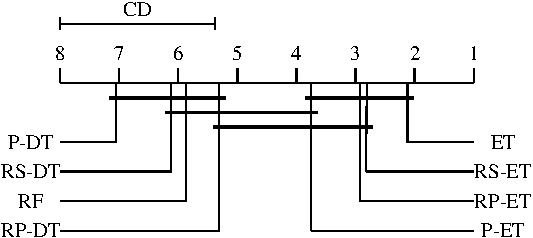
\includegraphics[width=0.9\textwidth]{figures/ch8_rank_small.pdf}
    \caption{Average ranks of all methods on small datasets.}
    \label{fig:8:small-cmp}
\end{figure}

\begin{table}
    \centering
    \footnotesize
  \begin{tabular}{|l|cccccccc|}
    \hline
         & RF & ET & P-DT & P-ET & RS-DT & RS-ET & RP-DT & RP-ET \\
    \hline
    \hline
        RF     &  ---   & 1/2/13 & 12/4/0  & 1/7/8   & 4/7/5   & 2/2/12 & 1/10/5  & 0/4/12 \\
        ET     &  13/2/1 & ---   & 14/1/1  & 10/5/1  & 13/3/0  & 4/11/1 & 12/2/2  & 5/10/1 \\
        P-DT   &  0/4/12 & 1/1/14 & ---    & 0/4/12  & 2/3/11  & 2/1/13 & 0/4/12  & 0/4/12 \\
        P-ET   &  8/7/1  & 1/5/10 & 12/4/0  & ---    & 9/6/1   & 2/6/8  & 9/6/1   & 0/11/5 \\
        RS-DT  &  5/7/4  & 0/3/13 & 11/3/2  & 1/6/9   & ---    & 0/2/14 & 1/11/4  & 0/4/12 \\
        RS-ET  &  12/2/2 & 1/11/4 & 13/1/2  & 8/6/2   & 14/2/0  & ---   & 11/4/1  & 1/13/2 \\
        RP-DT  &  5/10/1 & 2/2/12 & 12/4/0  & 1/6/9   & 4/11/1  & 1/4/11 & ---    & 0/6/10 \\
        RP-ET  &  12/4/0 & 1/10/5 & 12/4/0  & 5/11/0  & 12/4/0  & 2/13/1 & 10/6/0  & ---\\
    \hline
    \end{tabular}
    \caption{Pairwise t-test comparisons on small datasets.}
    \label{table:rp:small-ttest}
\end{table}

% ET versus DT

Since all methods are variants of ensembles of decision trees, average
accuracies are not strikingly different from one method to another (see Table 1
of the supplementary materials). Yet, significant trends appear when looking at
Figure \ref{fig:8:small-cmp} and Table \ref{table:rp:small-ttest}.  First, all ET-based
methods are ranked before DT-based methods, including the popular Random
Forest algorithm. Overall, the original ET algorithm is ranked first ($R_{ET} =
2.125$), then come RS-ET and RP-ET at close positions ($R_{RS-ET} = 2.8125$ and
$R_{RP-ET} = 2.9375$) while P-ET is a bit behind ($R_{P-ET} = 3.75$). According
to Figure \ref{fig:8:small-cmp}, only ET is ranked significantly higher than all
DT-based method but looking at Table \ref{table:rp:small-ttest}, the worse ET-based
variant (P-ET) is still 9 times significantly better (w.r.t. the 50
runs over each set) and only 1 times significantly worse than the best DT-based
variant (RP-DT). The separation between these two families of algorithm
thus appears quite significant. This observation clearly suggests that using
random split thresholds, instead of optimized ones like in decision trees, pays
off in terms of generalization.

% RP versus RS et P (ET)

Among ET-based methods, RP-ET is better than P-ET but it is superseded by ET and
RS-ET in terms of average rank. Since RS-ET is a particular case of RP-ET, this
suggests that we are slightly overfitting when tuning the additional parameter
$\alpha_s$. And indeed RP-ET is better ranked than RS-ET in average on the validation
set (results not shown). Table~\ref{table:rp:small-ttest} however indicates
otherwise and makes RP-ET appear as slightly better than RS-ET (2/13/1).
Regarding ET over RP-ET, the better performance of the former (5/10/1) is
probably due to the fact that in ET subsets of features are redrawn locally at
each node when building trees and not once and for all prior to their
construction. This gives less chances to generate improper trees because of a
bad initial choice of features and thus leads to a lower bias and a better
accuracy.

% RP versus RS et P (DT)

Among DT-based methods, RP-DT now comes first (mean rank of 5.3125),
then RF ($R_{RF} = 5.875$), RS-DT ($R_{RS-DT} = 6.125$) and then P-DT
in last ($R_{P-DT} = 7.0625$). RP is only significantly worse than
another DT-based variant on 1 dataset. The extra-randomization brought
by the random choices of both samples and features seems to be
beneficial with decision trees that do not benefit from the
randomization of discretization thresholds. The fact that RF samples
features locally does not appear here anymore as an advantage over RP
(RF is significantly worse on 5 problems and better on only one),
probably because the decrease of bias that it provides does not exceed
the increase of variance with respect to global feature selection.

\subsection{Larger datasets}

While the former experiments revealed promising results, it is fair to ask
whether the conclusions that have been drawn would hold on and generalize to
larger problems, for example when dealing with a few relevant features buried
into hundreds or thousands of not important features (e.g., in genomic data),
or when dealing with many correlated features (e.g., in images). To investigate
this question, a second bench of experiments was carried out on 13 larger
datasets (see Table~\ref{table:rp:large-data}). All but
\textsc{madelon} are real data. In terms of dimensions, these datasets are far bigger,
ranging from a few hundreds of samples and thousands of features, to thousands of
samples but hundreds of features. As such, the complexity of the problems is
expected to be greater.  We adopted the exact same protocol as for smaller
datasets. However, to lower computing times, for datasets marked with $*$, the
methods were run using 100 trees instead of 250 and the minimum number of
samples required in an internal node was set to 10 in order to control
complexity. Detailed results are provided in Table~\ref{table:rp:accuracy-large}
and are summarized in Figure \ref{fig:8:large-cmp} and
Table \ref{table:rp:large-ttest}, respectively in terms of average rank (the
critical difference at $\alpha=0.05$ is now 2.9120) and Win/Draw/Loss statuses
obtained with paired t-tests. A Friedman test (at $\alpha=0.05$) still
indicates that some methods are significantly different from the others.

\begin{table}
    \centering
    \footnotesize
    \begin{tabular}{| l | c c |}
    \hline
    \textbf{Dataset} & $N$ & $p$ \\
    \hline
    \hline
                \textsc{cifar10}*   & 60000   & 3072   \\
                \textsc{mnist3vs8}  & 13966   & 784    \\
                \textsc{mnist4vs9}  & 13782   & 784    \\
                \textsc{mnist}*     & 70000   & 784    \\
                \textsc{isolet}     & 7797    & 617    \\
                \textsc{arcene}     & 900     & 10000  \\
                \textsc{breast2}    & 295     & 24496  \\
                \textsc{madelon}    & 4400    & 500    \\
                \textsc{marti0}     & 500     & 1024   \\
                \textsc{reged0}     & 500     & 999    \\
                \textsc{secom}      & 1567    & 591    \\
                \textsc{tis}        & 13375   & 927    \\
                \textsc{sido0}*     & 12678   & 4932   \\
    \hline
    \end{tabular}
    \caption{Large datasets.}
    \label{table:rp:large-data}
\end{table}

\begin{table}
    \centering
    \footnotesize
    \hspace{-3.2cm}
\begin{tabular}{|l|cccccccc|}
\hline
\textbf{Validation} & RF & ET & P-DT & P-ET & RS-DT & RS-ET & RP-DT & RP-ET \\
\hline
\hline
    \textsc{cifar10 }  &  45.16 (6)  &  \textbf{46.17} (1)  &  44.92 (7)  &  44.88 (8)  &  45.83 (5)  &  46.09 (3)  &  45.89 (4)  &  46.13 (2) \\
    \textsc{mnist3v8}  &  98.42 (7)  &  98.77 (5)  &  97.63 (8)  &  98.57 (6)  &  98.79 (4)  &  98.86 (2)  &  98.81 (3)  &  \textbf{98.87} (1) \\
    \textsc{mnist4v9}  &  98.47 (7)  &  98.82 (3)  &  97.39 (8)  &  98.47 (6)  &  98.77 (5)  &  98.89 (2)  &  98.80 (4)  &  \textbf{98.91} (1) \\
    \textsc{mnist   }  &  96.14 (7)  &  96.56 (3)  &  94.35 (8)  &  96.19 (6)  &  96.52 (5)  &  96.57 (2)  &  96.53 (4)  &  \textbf{96.57} (1) \\
    \textsc{isolet  }  &  93.96 (7)  &  95.07 (3)  &  90.90 (8)  &  94.23 (6)  &  94.38 (5)  &  95.15 (2)  &  94.47 (4)  &  \textbf{95.20} (1) \\
    \textsc{arcene  }  &  73.84 (7)  &  77.76 (3)  &  73.76 (8)  &  75.12 (6)  &  76.40 (5)  &  77.60 (4)  &  79.44 (2)  &  \textbf{80.00} (1) \\
    \textsc{breast2 }  &  69.64 (6)  &  69.91 (4)  &  70.54 (3)  &  69.83 (5)  &  69.59 (7)  &  69.54 (8)  &  \textbf{72.59} (1)  &  71.62 (2) \\
    \textsc{madelon }  &  76.12 (8)  &  \textbf{81.41} (1)  &  78.48 (7)  &  81.06 (5)  &  80.68 (6)  &  81.29 (3)  &  81.18 (4)  &  81.36 (2) \\
    \textsc{marti   }  &  87.66 (8)  &  87.92 (6)  &  88.08 (4)  &  88.09 (3)  &  87.77 (7)  &  88.00 (5)  &  88.19 (2)  &  \textbf{88.20} (1) \\
    \textsc{reged   }  &  98.00 (6)  &  98.46 (2)  &  97.08 (8)  &  98.24 (5)  &  98.00 (7)  &  98.41 (3)  &  98.40 (4)  &  \textbf{98.57} (1) \\
    \textsc{secom   }  &  93.37 (5)  &  93.36 (6)  &  93.34 (8)  &  93.42 (2)  &  93.35 (7)  &  93.40 (4)  &  93.41 (3)  &  \textbf{93.45} (1) \\
    \textsc{tis     }  &  91.81 (5)  &  91.53 (7)  &  91.59 (6)  &  91.50 (8)  &  92.04 (3)  &  91.97 (4)  &  \textbf{92.26} (1)  &  92.06 (2) \\
    \textsc{sido    }  &  97.46 (5)  &  97.44 (6)  &  97.36 (8)  &  97.36 (7)  &  97.47 (3)  &  97.46 (4)  &  \textbf{97.52} (1)  &  97.52 (2) \\
\hline
\textit{Avg. rank} & 6.4615 & 3.8461 & 7.0   & 5.6153 & 5.3076 & 3.5384 &  2.8461 & 1.3846 \\
\hline
\hline
\textbf{Test} & RF & ET & P-DT & P-ET & RS-DT & RS-ET & RP-DT & RP-ET \\
\hline
\hline
    \textsc{cifar10 }  &  44.87 (7)  &  45.95 (2)  &  44.75 (8)  &  44.95 (6)  &  45.86 (4)  &  \textbf{46.02} (1)  &  45.74 (5)  &  45.93 (3) \\
    \textsc{mnist3v8}  &  98.31 (7)  &  98.64 (5)  &  97.47 (8)  &  98.48 (6)  &  98.70 (2)  &  \textbf{98.71} (1)  &  98.68 (4)  &  98.68 (3) \\
    \textsc{mnist4v9}  &  98.33 (6)  &  98.68 (2)  &  97.16 (8)  &  98.32 (7)  &  98.59 (4)  &  \textbf{98.69} (1)  &  98.59 (5)  &  98.67 (3) \\
    \textsc{mnist   }  &  96.10 (7)  &  96.47 (3)  &  94.30 (8)  &  96.18 (6)  &  96.47 (4)  &  \textbf{96.49} (1)  &  96.46 (5)  &  96.48 (2) \\
    \textsc{isolet  }  &  93.87 (7)  &  \textbf{94.95} (1)  &  90.71 (8)  &  94.15 (6)  &  94.33 (4)  &  94.94 (2)  &  94.29 (5)  &  94.88 (3) \\
    \textsc{arcene  }  &  71.04 (4)  &  \textbf{72.56} (1)  &  66.16 (8)  &  68.56 (7)  &  71.52 (3)  &  72.24 (2)  &  69.44 (6)  &  70.00 (5) \\
    \textsc{breast2 }  &  65.86 (6)  &  \textbf{66.16} (1)  &  65.54 (8)  &  65.59 (7)  &  66.13 (2)  &  65.91 (5)  &  65.94 (4)  &  66.08 (3) \\
    \textsc{madelon }  &  75.33 (8)  &  \textbf{80.83} (1)  &  77.86 (7)  &  80.78 (2)  &  80.06 (6)  &  80.59 (3)  &  80.06 (5)  &  80.42 (4) \\
    \textsc{marti   }  &  87.74 (8)  &  87.85 (6)  &  \textbf{88.24} (1)  &  88.17 (2)  &  87.82 (7)  &  88.06 (4)  &  88.08 (3)  &  88.01 (5) \\
    \textsc{reged   }  &  97.60 (5)  &  \textbf{98.20} (1)  &  96.40 (8)  &  97.92 (3)  &  97.39 (6)  &  98.00 (2)  &  97.32 (7)  &  97.82 (4) \\
    \textsc{secom   }  &  93.30 (7)  &  93.22 (8)  &  \textbf{93.38} (1)  &  93.30 (6)  &  93.37 (2)  &  93.31 (4)  &  93.33 (3)  &  93.31 (5) \\
    \textsc{tis     }  &  91.68 (5)  &  91.42 (7)  &  91.49 (6)  &  91.40 (8)  &  \textbf{92.05} (1)  &  91.91 (3)  &  92.05 (2)  &  91.90 (4) \\
    \textsc{sido    }  &  97.33 (4)  &  97.33 (3)  &  97.26 (7)  &  97.26 (8)  &  \textbf{97.35} (1)  &  97.34 (2)  &  97.33 (5)  &  97.32 (6) \\
\hline
\textit{Avg. rank} & 6.2307 & 3.1538 & 6.6153 & 5.6923 & 3.5384 & 2.3846 & 4.5384 & 3.8461 \\
\hline
\end{tabular}
    \caption{Accuracy on larger datasets (in \%).}
    \label{table:rp:accuracy-large}
\end{table}

As it may be observed from Figure~\ref{fig:8:large-cmp}, the average ranks of the
methods are closer to each other than in the previous experiments, now ranging
from 2.38 to 6.61, while they were previously ranging from 2.12 to 7. Methods
are more connected by critical difference bars. This suggests that overall they
behave more similarly to each other than before. General trends are nevertheless
comparable to what we observed earlier. ET-based methods still seem to be the
front-runners.  From Figure~\ref{fig:8:large-cmp}, RS-ET, ET and RP-ET are in the
top 4, while P-DT, RF and RP-DT remain in the second half of the ranking.
Surprisingly however, RS-DT now comes right after RS-ET and ET and just before
RP-ET whereas it ranked penultimate on the smaller datasets. Table~\ref{table:rp:large-ttest}
however suggests that RS-DT performs actually a little worse
against RP-ET (1/10/2).  All in all, it thus still seems beneficial to randomize
split thresholds on the larger datasets.

Comparing ET-based variants, ET is no longer the best method on average, but RS-ET
is (with 4/9/0 for RS-ET versus ET). This suggests than on larger datasets,
picking features globally at random prior to the construction of the trees is as
good, or even beat picking them locally at each node. Due to the quantitatively
larger number of samples in a patch, and also to the larger number of redundant
features expected in some large datasets (e.g., in \textsc{cifar10} or \textsc{mnist}), it is
indeed less likely to build improper trees with strong biases. As a result,
variance can be further decreased by sampling globally. In support of this
claim, on a few problems such as \textsc{arcene}, \textsc{breast2}, or \textsc{madelon} that contain many
irrelevant features, ET remains the best method. In that case, it is indeed more
likely to sample globally improper random patches, and hence to build improper
trees. The average rank of RP-ET suggests that it performs worse than RS-ET and
thus that there is some potential overfitting when tuning $\alpha_s$ in addition to
$\alpha_f$. This difference is however not confirmed in Table~\ref{table:rp:large-ttest}
where the accuracies of these two methods are shown to be never significantly
different (0/13/0). RP-ET is also on a perfect par with ET (1/11/1). Among DT-based variants,
RP-DT, which was the best performer on small datasets, is still
ranked above RF and P-DT, but it is now ranked below RS-DT with a win/draw/loss
of 0/11/2. This is again due to some overfitting.

While less conclusive than before, the results on larger datasets are
consistent with what we observed earlier. In particular, they indicate that
the Random Patches method (with ET) remains competitive with the best
performers.

\begin{figure}
    \centering
    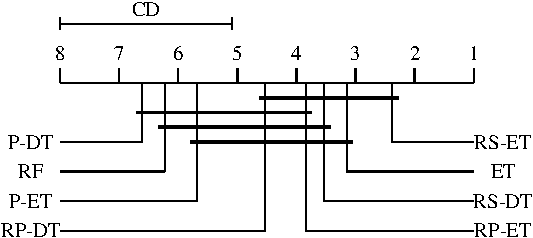
\includegraphics[width=0.9\textwidth]{figures/ch8_rank_large.pdf}
    \caption{Average ranks of all methods on larger datasets.}
    \label{fig:8:large-cmp}
\end{figure}

\begin{table}
    \centering
    \footnotesize
  \begin{tabular}{|l|cccccccc|}
    \hline
         & RF & ET & P-DT & P-ET & RS-DT & RS-ET & RP-DT & RP-ET \\
    \hline
    \hline
                RF     & ---    & 1/5/7   & 8/3/2  & 2/6/5  & 0/6/7  & 0/5/8  & 0/6/7  & 0/6/7 \\
                ET     & 7/5/1   & ---    & 9/2/2  & 7/6/0  & 3/7/3  & 0/9/4  & 5/6/2  & 1/11/1 \\
                P-DT   & 2/3/8   & 2/2/9   & ---   & 1/5/7  & 0/3/10 & 0/3/10 & 1/3/9  & 0/4/9 \\
                P-ET   & 5/6/2   & 0/6/7   & 7/5/1  & ---   & 0/6/7  & 0/5/8  & 2/5/6  & 1/5/7 \\
                RS-DT  & 7/6/0   & 3/7/3   & 10/3/0 & 7/6/0  & ---   & 1/8/4  & 2/11/0 & 1/10/2 \\
                RS-ET  & 8/5/0   & 4/9/0   & 10/3/0 & 8/5/0  & 4/8/1  & ---   & 4/8/1  & 0/13/0 \\
                RP-DT  & 7/6/0   & 2/6/5   & 9/3/1  & 6/5/2  & 0/11/2 & 1/8/4  & ---   & 1/9/3 \\
                RP-ET  & 7/6/0   & 1/11/1  & 9/4/0  & 7/5/1  & 2/10/1 & 0/13/0 & 3/9/1  & ---\\
    \hline
    \end{tabular}
    \caption{Pairwise t-test comparisons on larger datasets.}
    \label{table:rp:large-ttest}
\end{table}

\subsection{Conclusions}

Overall, this extensive experimental study reveals many interesting results. The
first and foremost result is that ensembles of randomized trees nearly always
beat ensembles of standard decision trees. As off-the-shelf methods, we advocate
that ensembles of such trees should be preferred to ensembles of decision trees.
In particular, these results show that the well-known Random Forest algorithm
does not compete with the best performers.  Far more important to our concern
though, this study validates our RP approach. Building ensembles (of ET) on
random patches of data is competitive in terms of accuracy. Overall, there is no
strong statistical evidence that the method performs less well, but there is
also no conclusive evidence that it significantly improves performance. Yet,
results show that RP is often as good as the very best methods. Regarding the
shape of the random patches, the strategy behind Pasting (i.e., $\alpha_s$ free and
$\alpha_f=1.0$) proved to be (very) ineffective on many datasets while the Random
Subspace algorithm (i.e., $\alpha_s=1.0$ and $\alpha_f$ free) always ranked among the very
best performers. On average, RS indeed came in second on the small datasets and
in first on the larger datasets, which tends to indicate that sampling features
is crucial in terms of accuracy. As for patches of freely adjustable size (i.e.,
using RP), they showed to be slightly sensitive to overfitting but proved to
remain closely competitive with the very best methods. In addition, these
results also suggest that sampling features globally, once and for all, prior to
the construction of a (randomized) decision tree, does not actually impair
performance. For instance, RS-ET or RP-ET are indeed not strongly worse, nor
better, than ET, in which candidates features are re-sampled locally at each
node.

\section{On Memory}
\label{sec:9:memory}

Section~\ref{sec:9:accuracy} reveals that building an ensemble of base
estimators on random patches, instead of the whole data, is a competitive
strategy. In the context of big data, that is when the size of the dataset is
far bigger than the available memory, this suggests that using  random
parts of the data of the appropriate size to build each base estimator would
likely result in an ensemble which is actually as good as if the whole data
could have been loaded and used.

Formally, we assume a general framework where the number of data units that can
be loaded at once into memory is constrained to be lower than a given threshold
$\mu_{\text{max}}$. Not considering on-line algorithms within the scope of this study,
$\mu_{\text{max}}$ can hence be viewed as the total units of data allowed to be used to
build a single base estimator. In the context of our sampling methods, the
amount of memory required for a patch is given by $(\alpha_s N)(\alpha_f p)$ and thus
constraining memory by $\mu_{\text{max}}$ is equivalent to constraining the relative
patch size $\alpha_s\alpha_f$ to be lower than $\mu'_{\text{max}}=\mu_{\text{max}}/(Np)$. While
simplistic\footnote{e.g., the quantity of memory used by the estimator itself
  is not taken into account.}, this framework has the advantage of clearly
addressing one of the main difficulties behind big data, that is the lack of
fast memory. Yet, it is also relevant in other contexts, for example when data
is costly to access (e.g., on remote locations) or when algorithms are run on embedded systems
with strong memory constraints.

In Section \ref{sec:9:memory:sensitivity}, we first study the effects of $\alpha_s$
and $\alpha_f$ on the accuracy of the resulting ensemble and show that it is problem
and base estimator dependent. Second, we show that the memory requirements,
i.e., the relative size $\alpha_s \alpha_f$ of the random patches, can often be
drastically reduced without significantly degrading the performance of the
ensemble (Section \ref{sec:9:memory:noloss}). Third, because the sensitivity of
the ensemble to $\alpha_s$ and $\alpha_f$ is problem and base estimator specific, we show
that under very strong memory constraints adjusting both parameters at the same
time, as RP does, is no longer merely as good but actually significantly better
than other ensemble methods (Section \ref{sec:9:memory:loss}).

\subsection{Sensitivity to $\alpha_s$ and $\alpha_f$}
\label{sec:9:memory:sensitivity}

Let us first consider and analyze the triplets
\begin{equation}
\{(\alpha_s, \alpha_f, \text{Acc}_{\cal L}(\alpha_s,\alpha_f)) | \forall \alpha_s, \alpha_f\}
\end{equation} for various problems, where $\text{Acc}_{\cal L}(\alpha_s,\alpha_f)$ is the average
test accuracy of an ensemble built on random patches of size $\alpha_s \alpha_f$ (using
the same protocol as previously) on the dataset ${\cal L}$.

As Figure~\ref{fig:9:surfaces} illustrates for six datasets, the
surfaces defined by these points vary significantly from one problem to
another. We observed four main trends. In Figures \ref{fig:surfaces:arcene},
and \ref{fig:surfaces:cifar10} (resp., \ref{fig:surfaces:tis}), accuracy
increases with $\alpha_s$ (resp., $\alpha_f$) while adjusting $\alpha_f$ (resp., $\alpha_s$) has no
or limited impact. In Figure \ref{fig:surfaces:madelon}, the best strategy is
to increase both $\alpha_s$ and $\alpha_f$. Finally, in Figures \ref{fig:surfaces:isolet}
and \ref{fig:surfaces:mnist}, the surface features plateaus, which means that
beyond some threshold, increasing $\alpha_s$ or $\alpha_f$ does not yield any significant
improvement. Interestingly, in most of the cases, the optimum corresponds to a
value $\alpha_s\alpha_f$ much smaller than 1.

\begin{figure}
\begin{center}
        \subfloat[\textsc{arcene} (RP-ET)]{
            \label{fig:surfaces:arcene}
            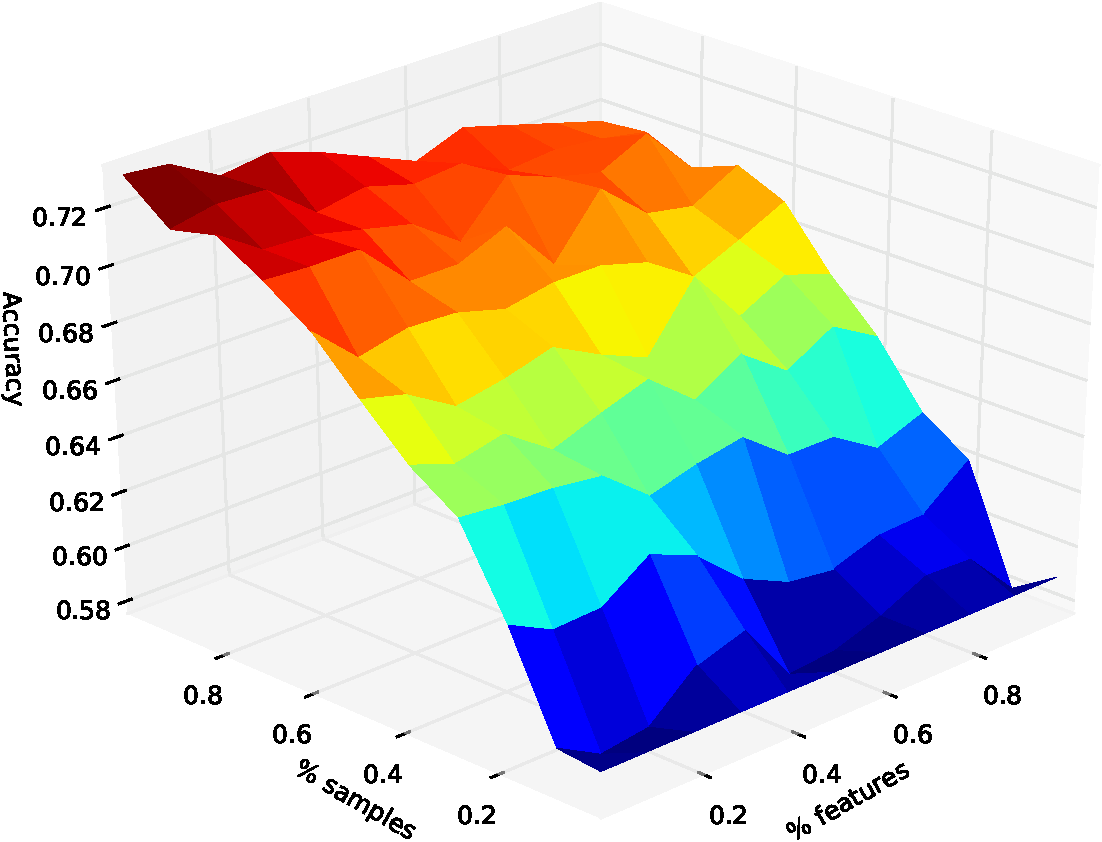
\includegraphics[width=0.31\textwidth]{figures/ch8/figure3-a-arcene-rp-et.pdf}
        }
        \subfloat[\textsc{cifar10} (RP-ET)]{
            \label{fig:surfaces:cifar10}
            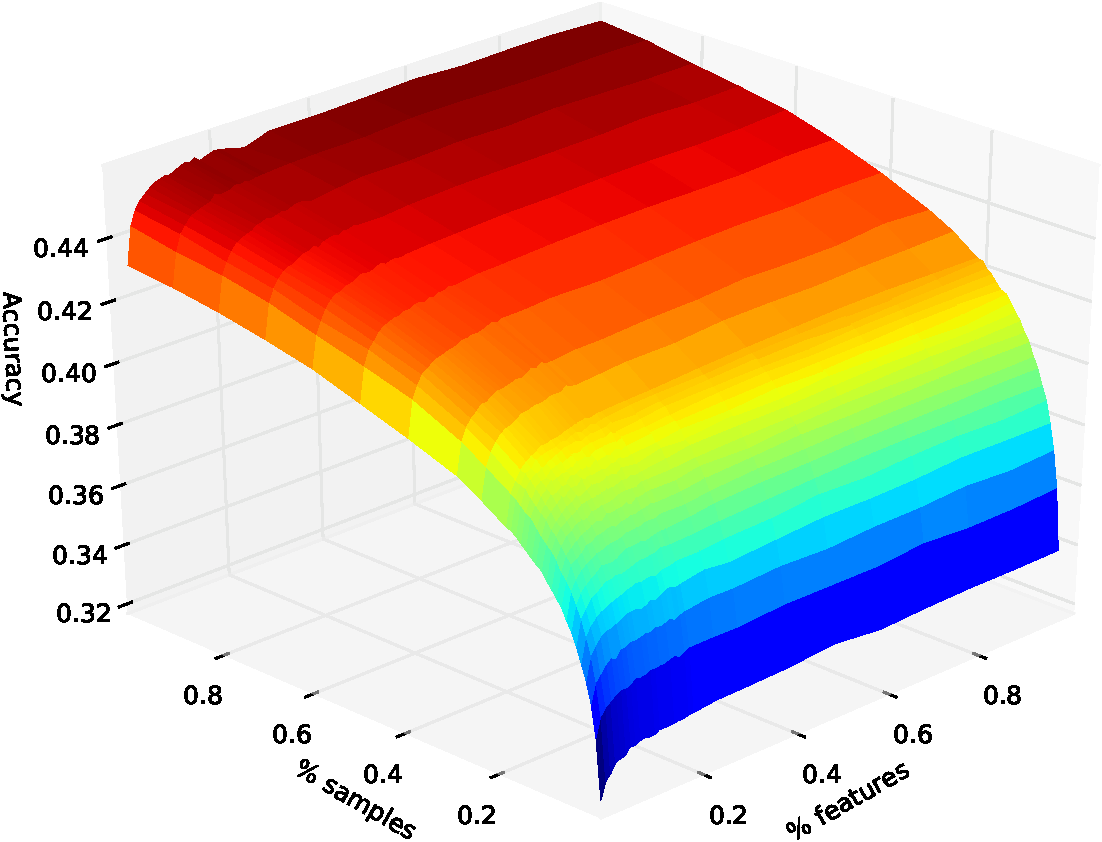
\includegraphics[width=0.31\textwidth]{figures/ch8/figure3-b-cifar10-rp-et.pdf}
        }
        \subfloat[\textsc{tis} (RP-ET)]{
            \label{fig:surfaces:tis}
            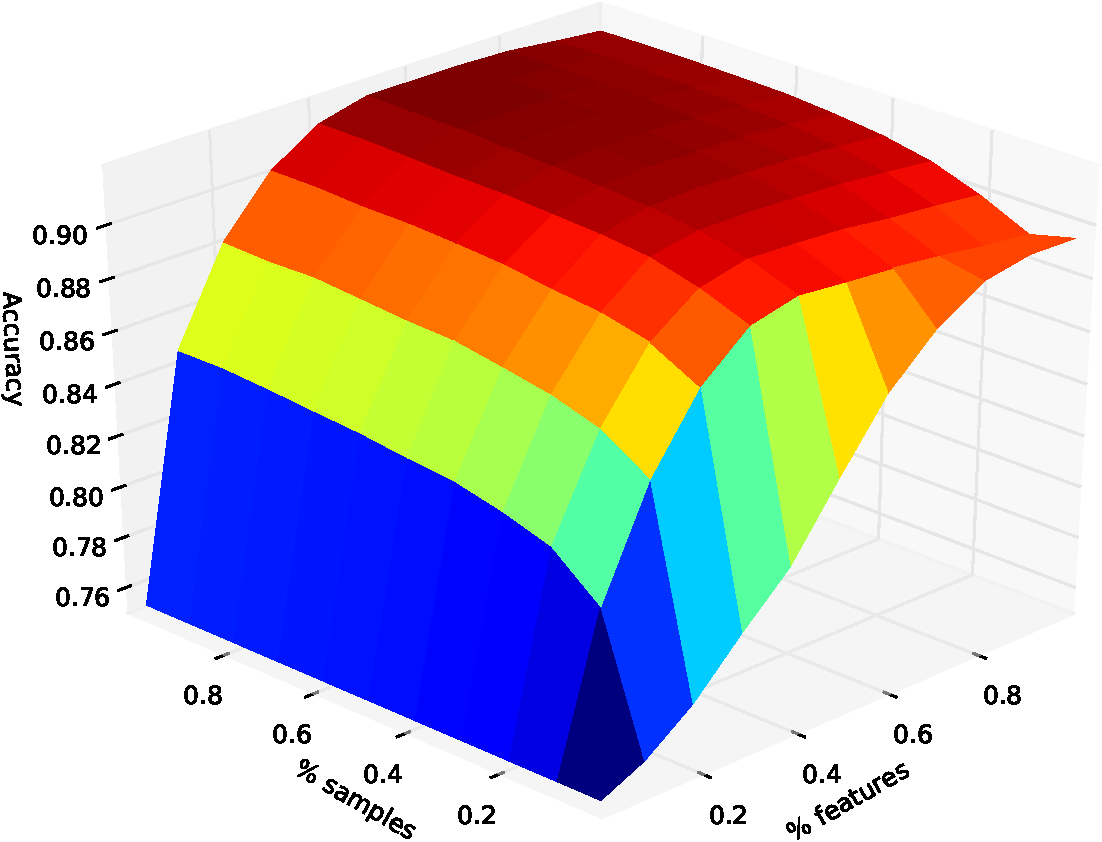
\includegraphics[width=0.31\textwidth]{figures/ch8/figure3-c-tis-rp-et.pdf}
        }

        \setcounter{subfigure}{0}
        \subfloat[\textsc{arcene} (RP-DT)]{
            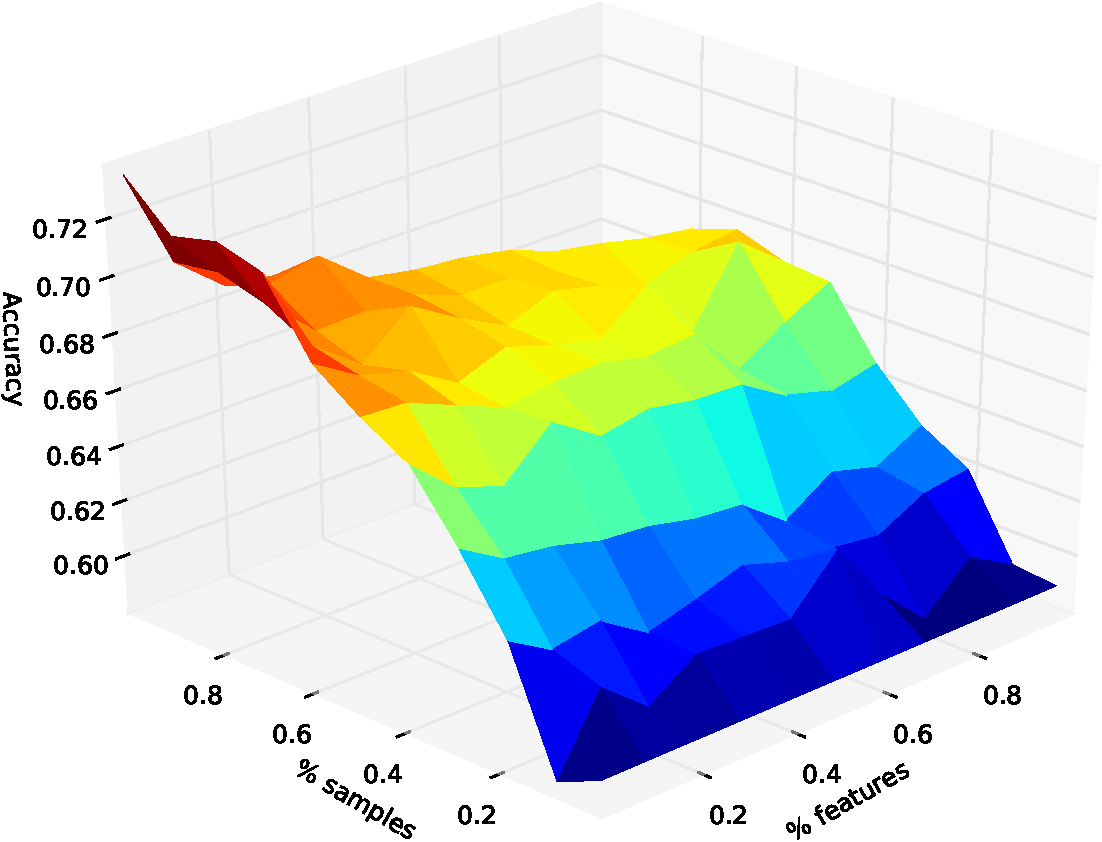
\includegraphics[width=0.31\textwidth]{figures/ch8/figure3-a-arcene-rp-dt.pdf}
        }
        \subfloat[\textsc{cifar10} (RP-DT)]{
            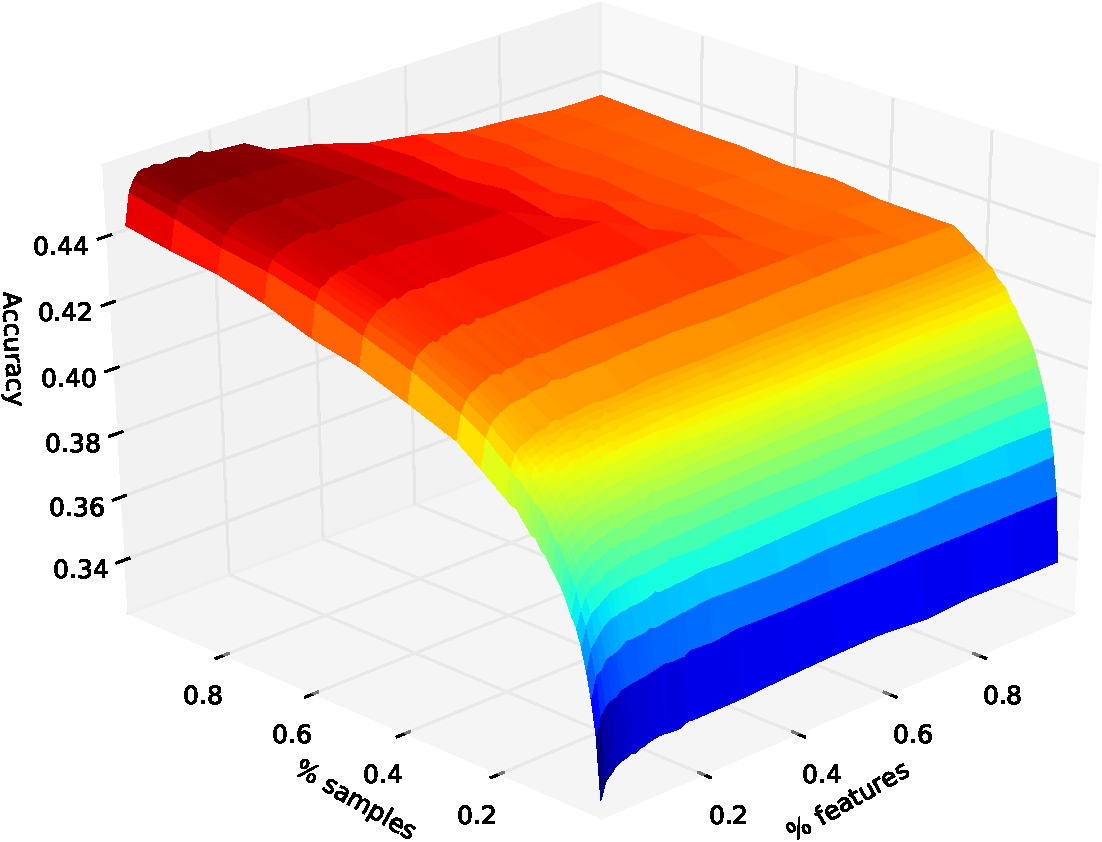
\includegraphics[width=0.31\textwidth]{figures/ch8/figure3-b-cifar10-rp-dt.pdf}
        }
        \subfloat[\textsc{tis} (RP-DT)]{
            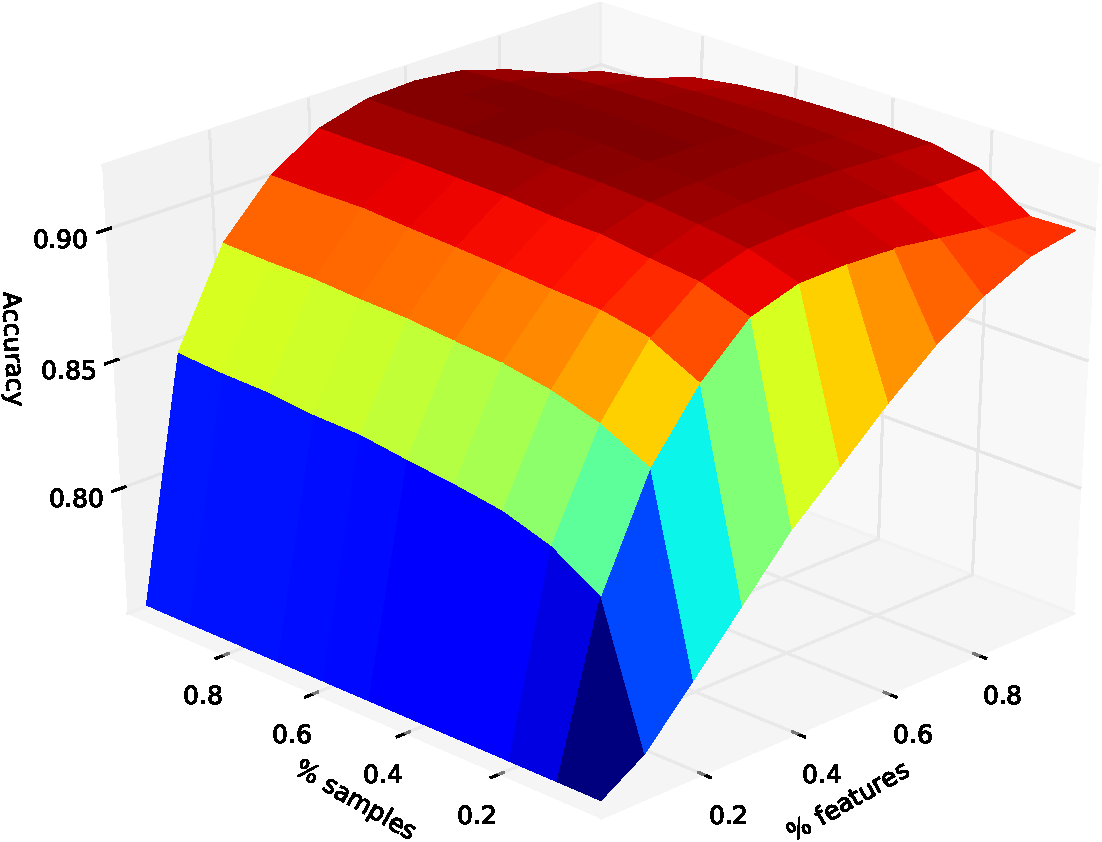
\includegraphics[width=0.31\textwidth]{figures/ch8/figure3-c-tis-rp-dt.pdf}
        }


        \subfloat[\textsc{madelon} (RP-ET)]{
            \label{fig:surfaces:madelon}
            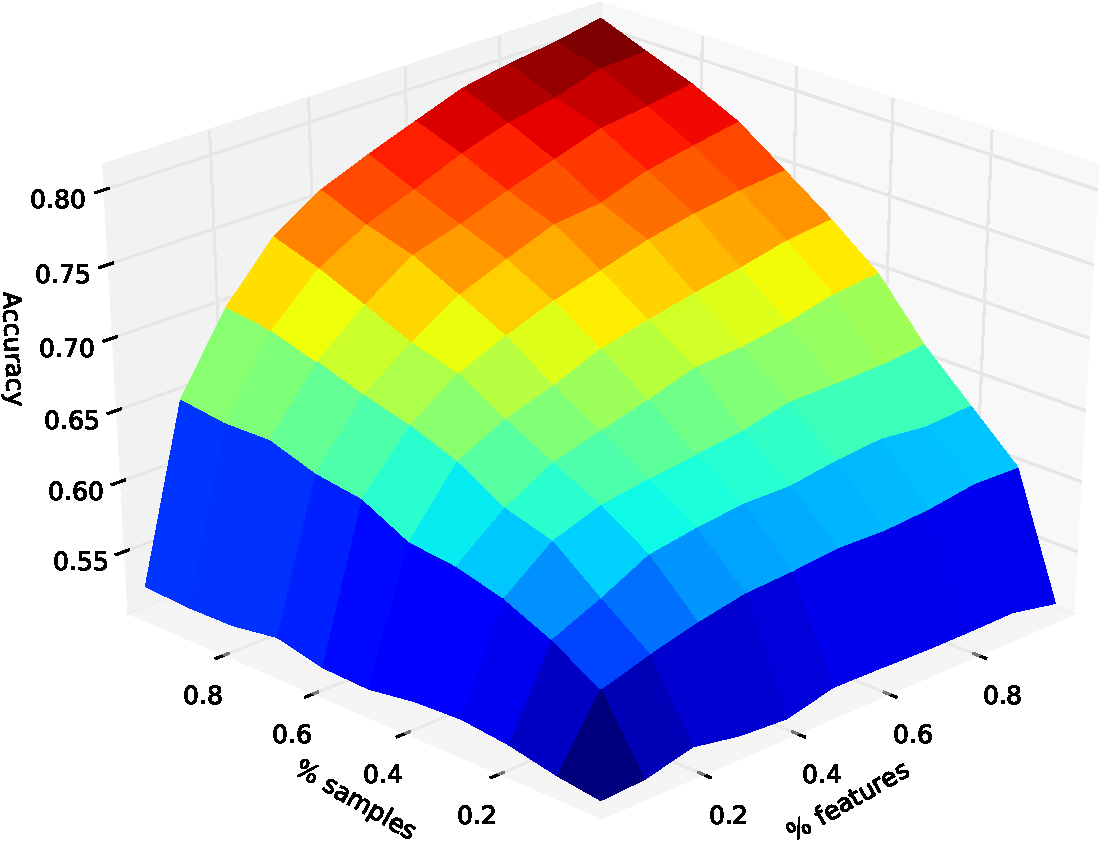
\includegraphics[width=0.31\textwidth]{figures/ch8/figure3-d-madelon-rp-et.pdf}
        }
        \subfloat[\textsc{isolet} (RP-ET)]{
            \label{fig:surfaces:isolet}
            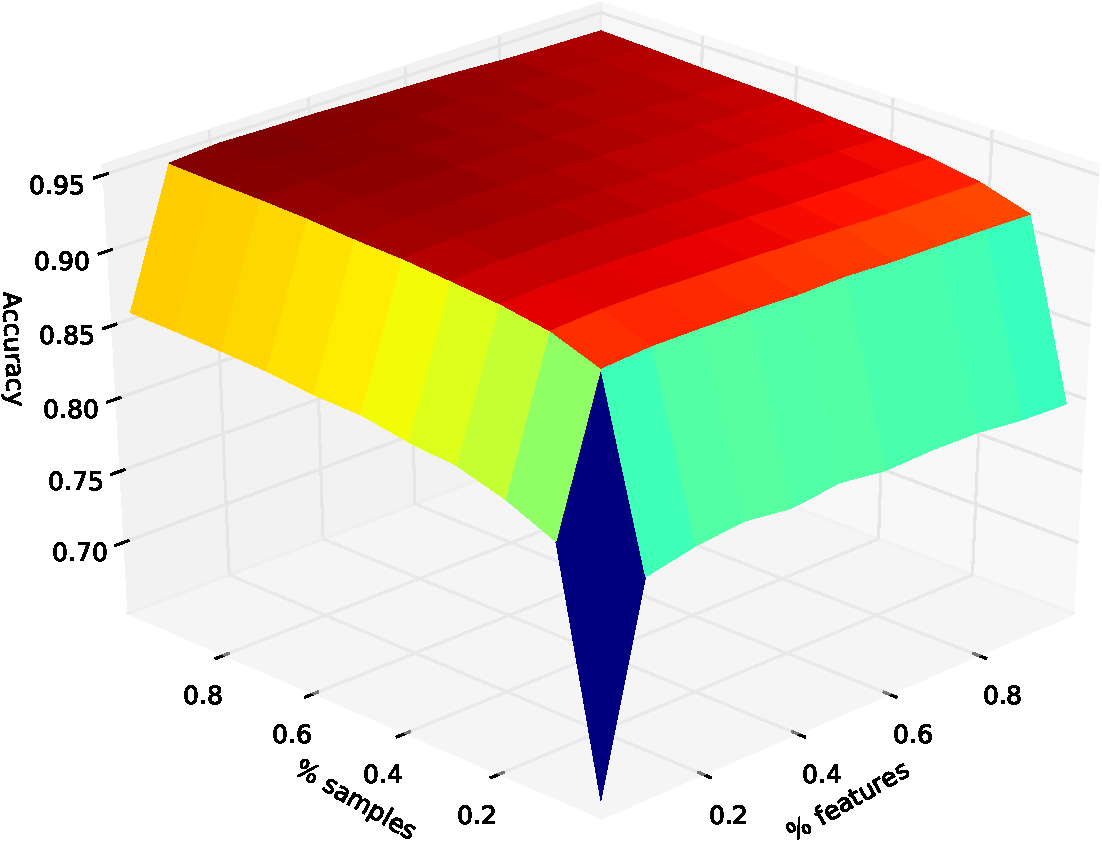
\includegraphics[width=0.31\textwidth]{figures/ch8/figure3-e-isolet-rp-et.pdf}
        }
        \subfloat[\textsc{mnist3vs8} (RP-ET)]{
            \label{fig:surfaces:mnist}
            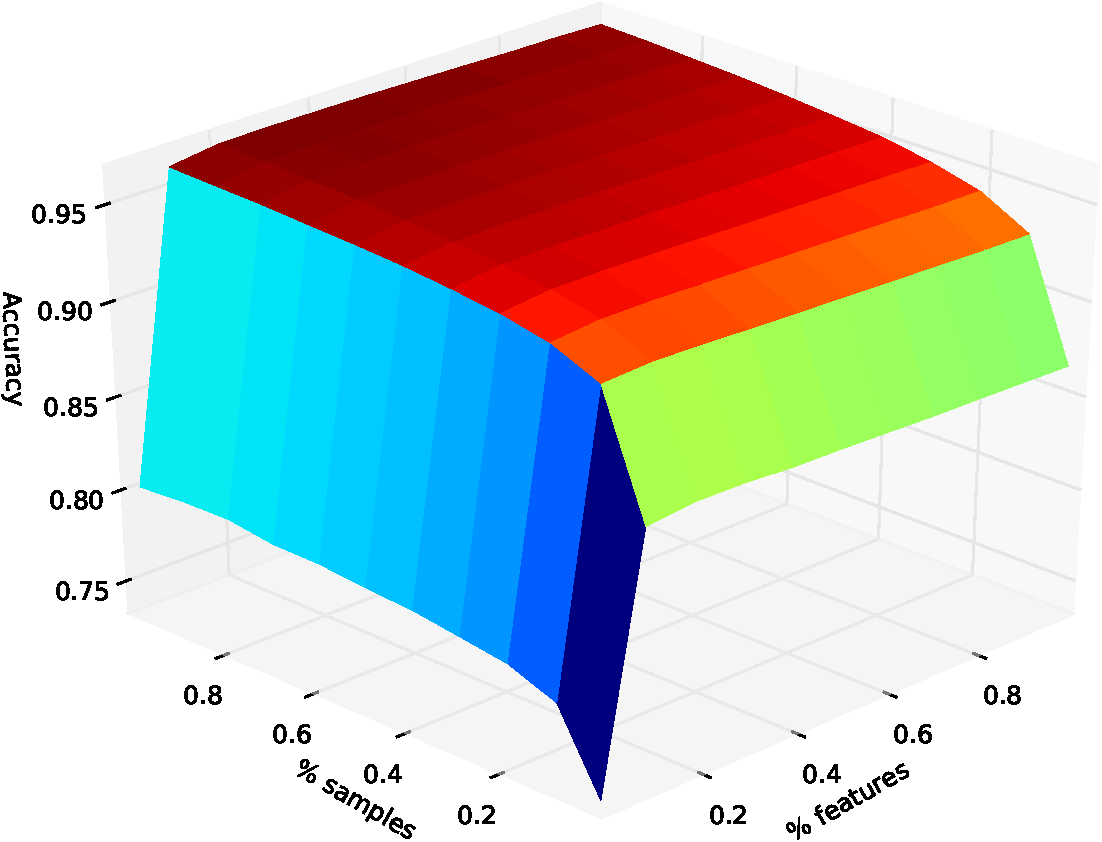
\includegraphics[width=0.31\textwidth]{figures/ch8/figure3-f-mnist-rp-et.pdf}
        }

        \setcounter{subfigure}{3}
        \subfloat[\textsc{madelon} (RP-DT)]{
            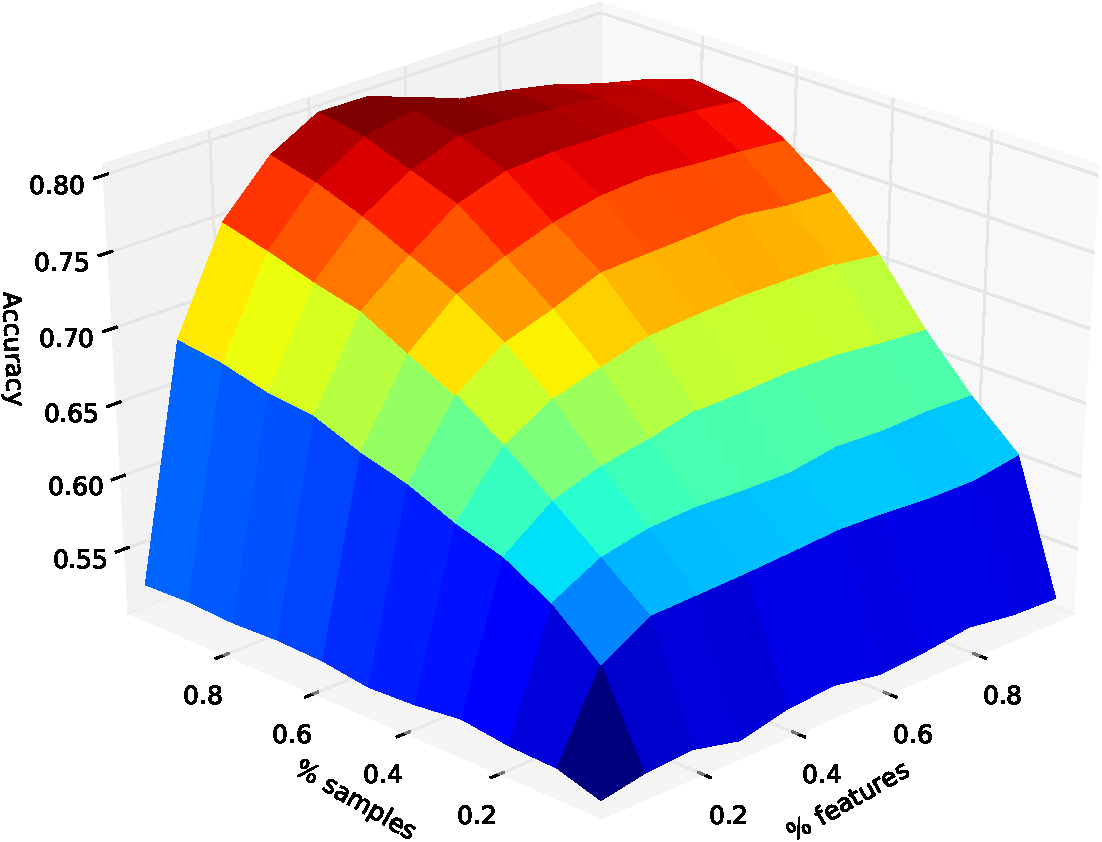
\includegraphics[width=0.31\textwidth]{figures/ch8/figure3-d-madelon-rp-dt.pdf}
        }
        \subfloat[\textsc{isolet} (RP-DT)]{
            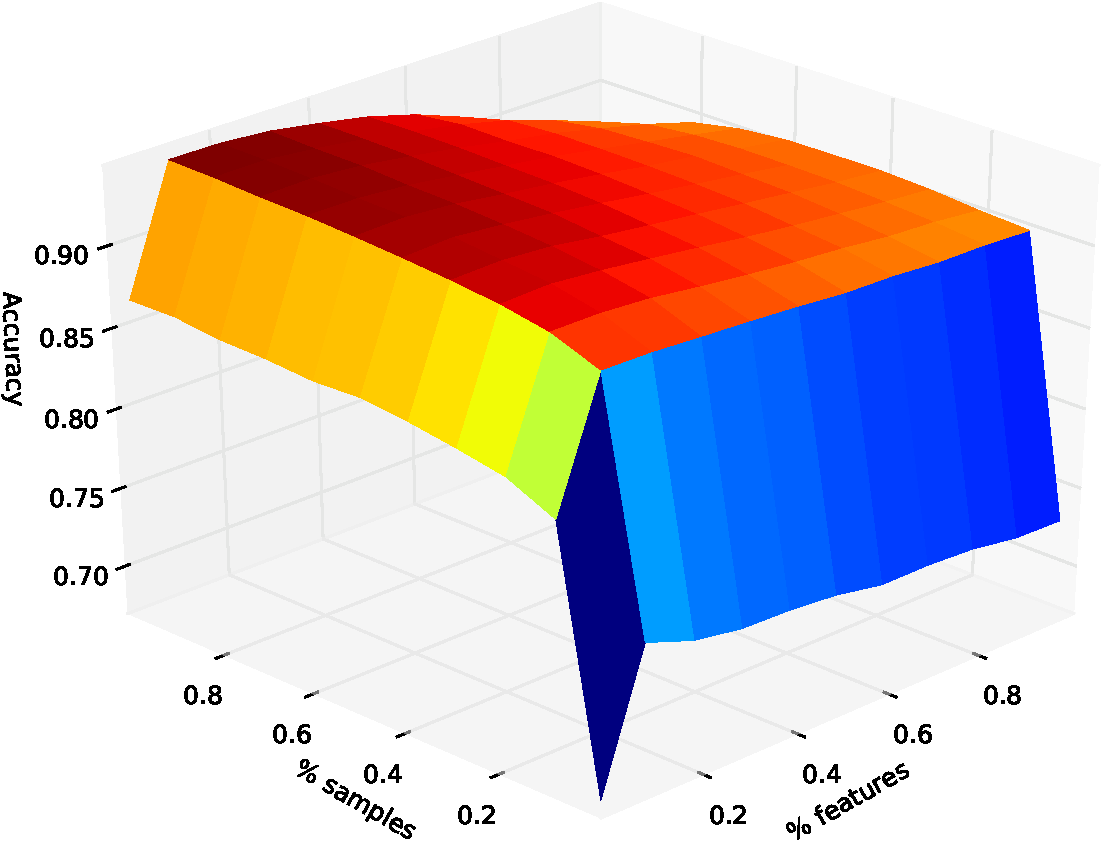
\includegraphics[width=0.31\textwidth]{figures/ch8/figure3-e-isolet-rp-dt.pdf}
        }
        \subfloat[\textsc{mnist3vs8} (RP-DT)]{
            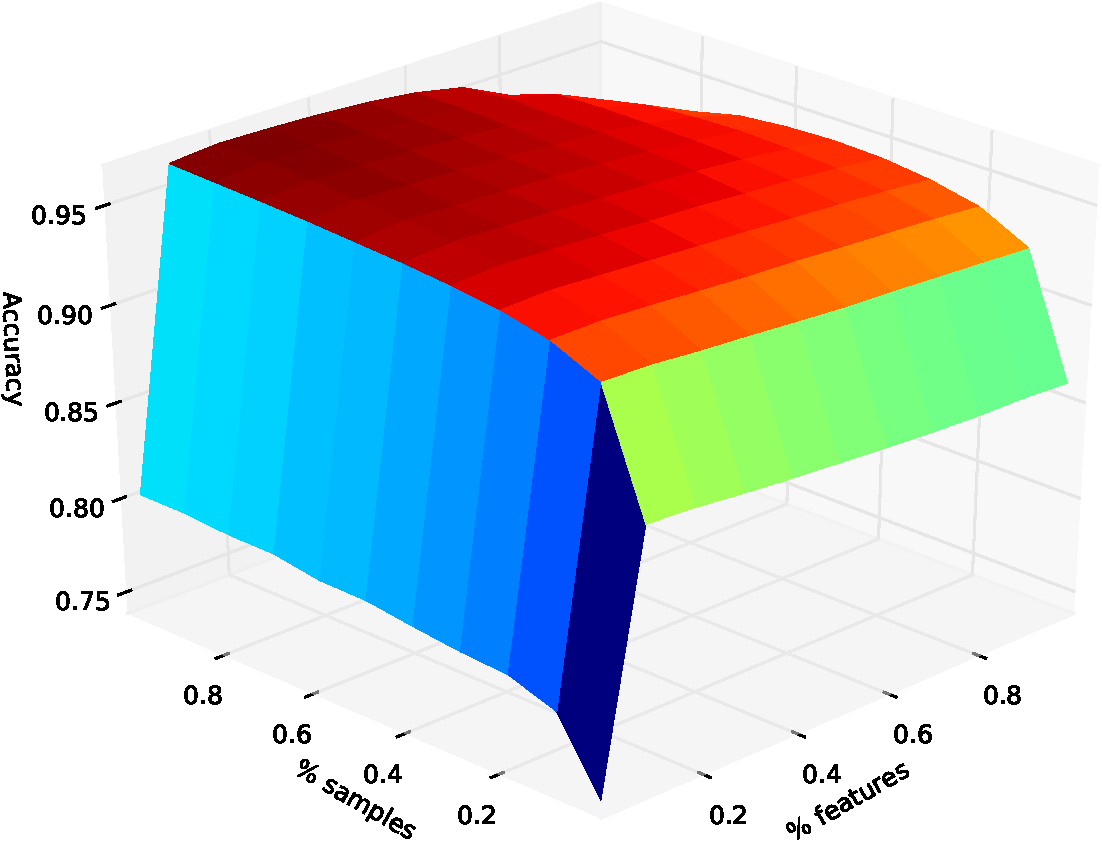
\includegraphics[width=0.31\textwidth]{figures/ch8/figure3-f-mnist-rp-dt.pdf}
        }
\caption{Learning surfaces.}
\label{fig:9:surfaces}
\end{center}
\end{figure}

The choice of the base estimators does not have a strong impact on the aspect
of the curves (compare the 1$^{st}$ and 3$^{rd}$ rows of sub-figures in
Figure~\ref{fig:9:surfaces} with those in the 2$^{nd}$ and 4$^{th}$ rows). The only
difference is the decrease of the accuracy of RP-DT when $\alpha_s$ and
$\alpha_f$ grow towards $1.0$. Indeed, since the only source of randomization in RP-DT
is patch selection, it yields in this case ensembles of identical
trees and therefore amounts to build a single tree on the whole
dataset. By contrast, because of the extra-randomization of the split
thresholds in ET, there is typically no drop of accuracy for RP-ET when $\alpha_s$
and $\alpha_f$ grow to $1.0$.

Overall, this analysis suggests that not only the best pair $\alpha_s \alpha_f$ depends
on the problem, but also that the sensitivity of the ensemble to changes to the
size of a random patch is both problem and base estimator specific. As a
result, these observations advocate for a method that could
favor $\alpha_s$, $\alpha_f$ or both, and do so
appropriately given the base estimator.

\subsection{Memory reduction, without significant loss}
\label{sec:9:memory:noloss}

We proceed to study in this section the actual size of the random patches when
the values of $\alpha_s$ and $\alpha_f$ are tuned using an independent validation
set. Our results are summarized in Figure~\ref{fig:9:memory:original}. Each
ellipse corresponds to one of the 29 datasets of our benchmark, whose center is
located at $(\overline{\alpha_s}, \overline{\alpha_f})$ (i.e., the average parameter
values over the 50 runs) and whose semi-axes correspond to the standard
deviations of $\alpha_s$ and $\alpha_f$. Any point in the plot corresponds to a pair
$(\alpha_s, \alpha_f)$ and thus to a relative consumption $\mu' = \alpha_s \alpha_f$ of memory. To
ease readability, level curves are plotted for $\mu' = 0.01, 0.1, ..., 0.9$. In
the right part of the figure, the histogram counts the number of datasets such
that $\overline{\alpha_s}\cdot\overline{\alpha_f}$ falls in the corresponding level set.

Figure~\ref{fig:9:memory:original} corroborates our previous discussion. On some
datasets, it is better to favor $\alpha_s$ while on some other increasing $\alpha_f$ is
a better strategy. The various sizes of the ellipses also confirm that the
sensitivity to variations of $\alpha_s$ and $\alpha_f$ is indeed problem-specific. The
figure also clearly highlights the fact that, even under no memory constraint, the
optimal patches rarely consume the whole memory. A majority of ellipses indeed
lie below the level set $\mu'=0.5$ and only a couple of them are above
$\mu'=0.75$. With respect to ET or RF for which the base estimators are all built
on the whole dataset, this means that ensembles of patches are not only as
competitive but also less memory greedy. In addition, the figure also
points out the difference between RP-ET and RP-DT as discussed in the previous
section. To ensure diversity, RP-DT is constrained to use smaller patches than
RP-ET, hence explaining why the ellipses in red are on average below those in
blue. While RP-DT proved to be a bit less competitive in terms of accuracy,
this indicates on the other hand that RP-DT may actually be more interesting
from a memory consumption point of view.

\begin{figure}
\begin{center}
        \subfloat[Original patches]{
            \label{fig:9:memory:original}
            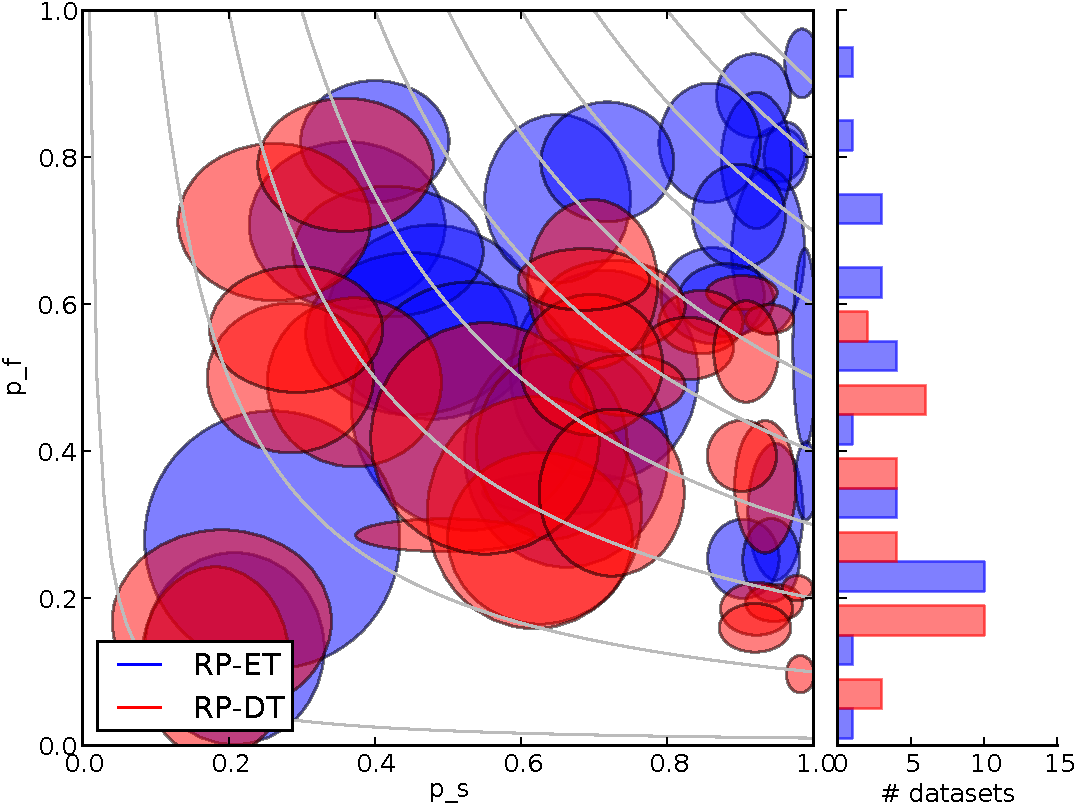
\includegraphics[width=0.5\textwidth]{figures/ch8/figure4-none.pdf}
        }
        \subfloat[Reduced patches]{
            \label{fig:9:memory:opt}
            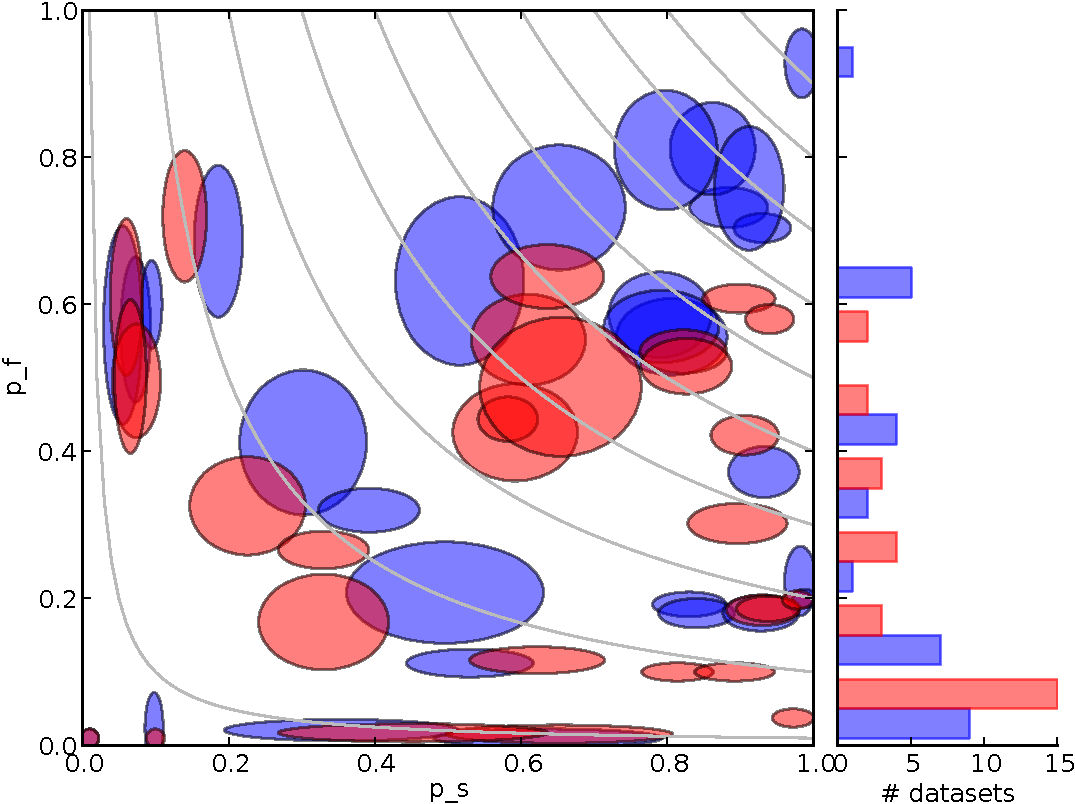
\includegraphics[width=0.5\textwidth]{figures/ch8/figure4-mem.pdf}
        }
\caption{Optimal sizes of the random patches on our benchmark.}
\label{fig:9:memory}
\end{center}
\end{figure}

In Section~\ref{sec:9:memory:sensitivity}, we observed plateaus or very
gentle slopes around the optimal pair $(\alpha_s, \alpha_f)$.  From a memory point of
view, this suggests that the random patches are likely to be reducible without
actually degrading the accuracy of the resulting ensemble. Put otherwise, our
interest is to find the smallest size $\alpha_s \alpha_f$ such that the accuracy of the
resulting ensemble is not significantly worse than an ensemble built without
such constraint. To that end, we study the extent at which the constraint $\alpha_s
\alpha_f < \mu'_{\text{max}}$ can be strengthened without any significant drop in
accuracy. If $\mu'_{\text{max}}$ can be reduced significantly then it would indeed mean that
even when only small parts of the data are actually used to build single base
estimators, competitive performance can still be achieved.

Figure~\ref{fig:9:memory:opt} summarizes our results. For all datasets, $\mu'_{\text{max}}$
was set to the lowest value such that it cannot be statistically detected that
the average accuracy of the resulting ensemble is different from the average
accuracy of an ensemble built with no memory constraint (at $\alpha=0.05$). With
regard to Figure~\ref{fig:9:memory:original}, the shift of most ellipses to lower
memory level sets confirm our first intuition. In many cases, the size of the
random patches can indeed be reduced, often drastically, without significant
decrease of accuracy. For more than half of the datasets, memory can indeed be
decreased to $\mu'=0.1$ or $\mu'=0.2$. In other words, building trees on small parts
of the data (i.e., $10\%$ or $20\%$ of the original dataset) is, for more than
half of the datasets, enough to reach competitive accuracy. Also, the
sensitivity to $\alpha_s$ and $\alpha_f$ is now even more patent. Some ensembles use very
few samples ($\alpha_s < 0.1$) but with many features, while other uses many samples
with few features ($\alpha_f < 0.1$). Again, from a memory point of view, RP-DT
appears to be more interesting than RP-ET. The memory reduction is larger, as
the histogram indicates. Optimized splits in the decision trees may indeed lead
to a better exploitation of the data, hence to a potentially larger reduction of
memory. In conclusion, while not detecting significant differences in accuracy
does not allow to conclude that the performances are truly similar, these
figures at least illustrate that memory requirements can be drastically reduced
without apparent loss in accuracy.

\subsection{Memory reduction, with loss}
\label{sec:9:memory:loss}

The previous section has shown that the memory consumption can be reduced up to
some threshold $\mu'_{\text{max}}$ with no significant loss in accuracy. In this section we
now look at the accuracy of the resulting ensemble when $\mu'_{\text{max}}$ is further
decreased. We argue that with severe constraints, and because datasets have all a
different sensitivity, it is even more crucial to better exploit data and thus
to find the right trade-off between both $\alpha_s$ and $\alpha_f$, as only RP can.

\begin{figure}
\begin{center}
        \subfloat[\textsc{arcene}]{
        \label{fig:memc:arcene}
            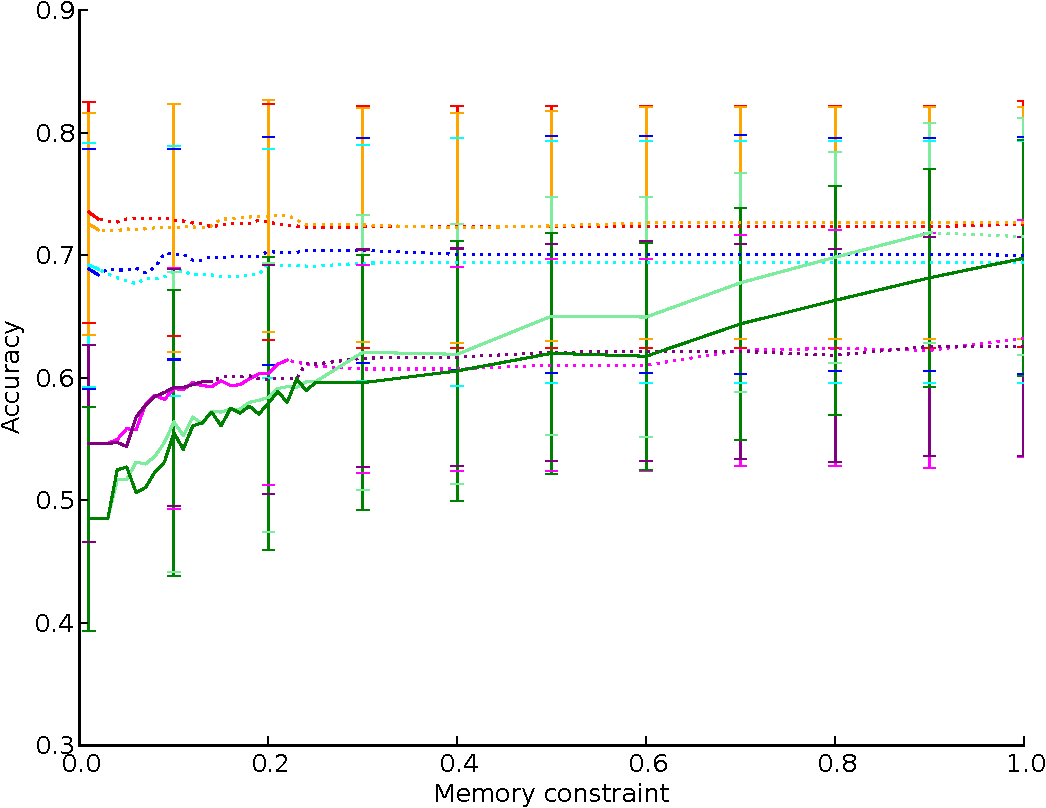
\includegraphics[width=0.5\textwidth]{figures/ch8/figure5-a-arcene.pdf}
        }
        \subfloat[\textsc{cifar10}]{
        \label{fig:memc:cifar10}
            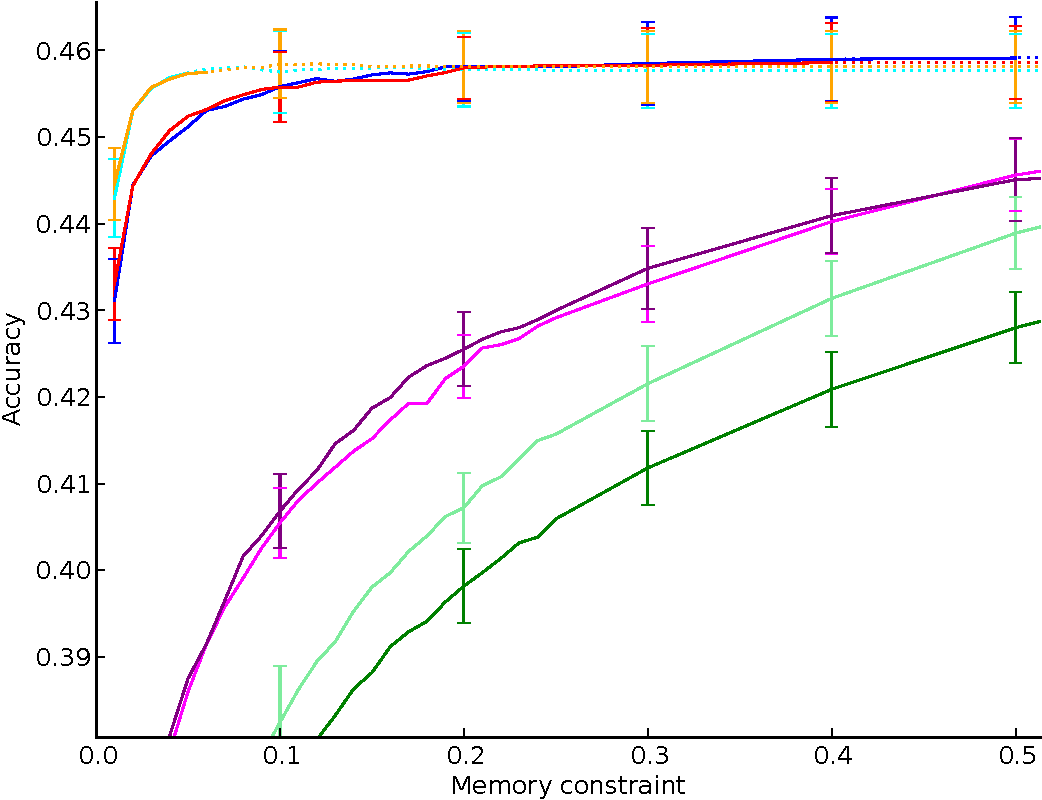
\includegraphics[width=0.5\textwidth]{figures/ch8/figure5-b-cifar10.pdf}
        }

        \subfloat[\textsc{tis}]{
        \label{fig:memc:tis}
            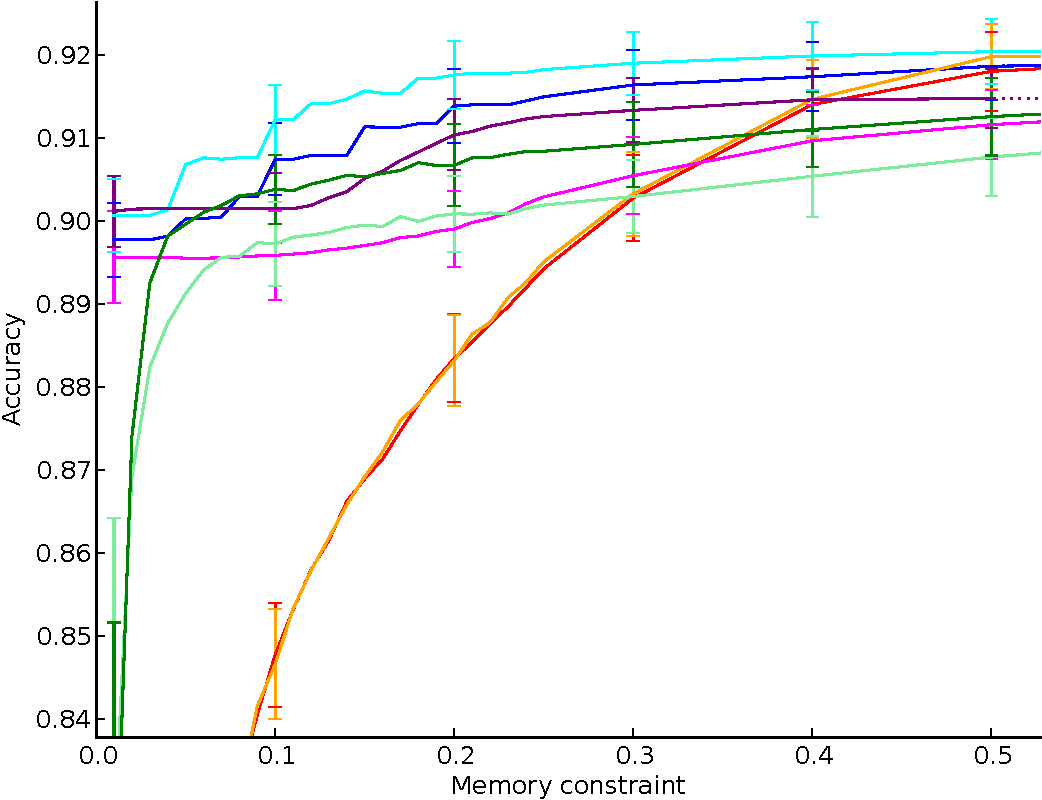
\includegraphics[width=0.5\textwidth]{figures/ch8/figure5-c-tis.pdf}
        }
        \subfloat[\textsc{madelon}]{
        \label{fig:memc:madelon}
            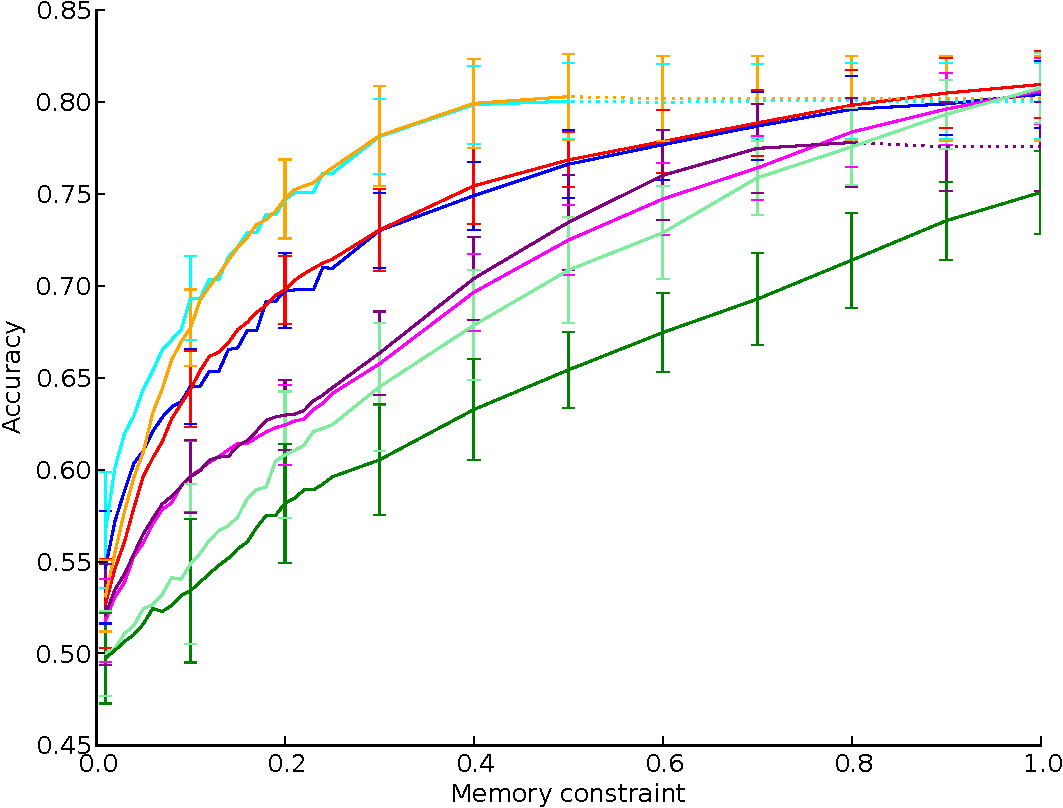
\includegraphics[width=0.5\textwidth]{figures/ch8/figure5-d-madelon.pdf}
        }

        \subfloat[\textsc{isolet}]{
        \label{fig:memc:isolet}
            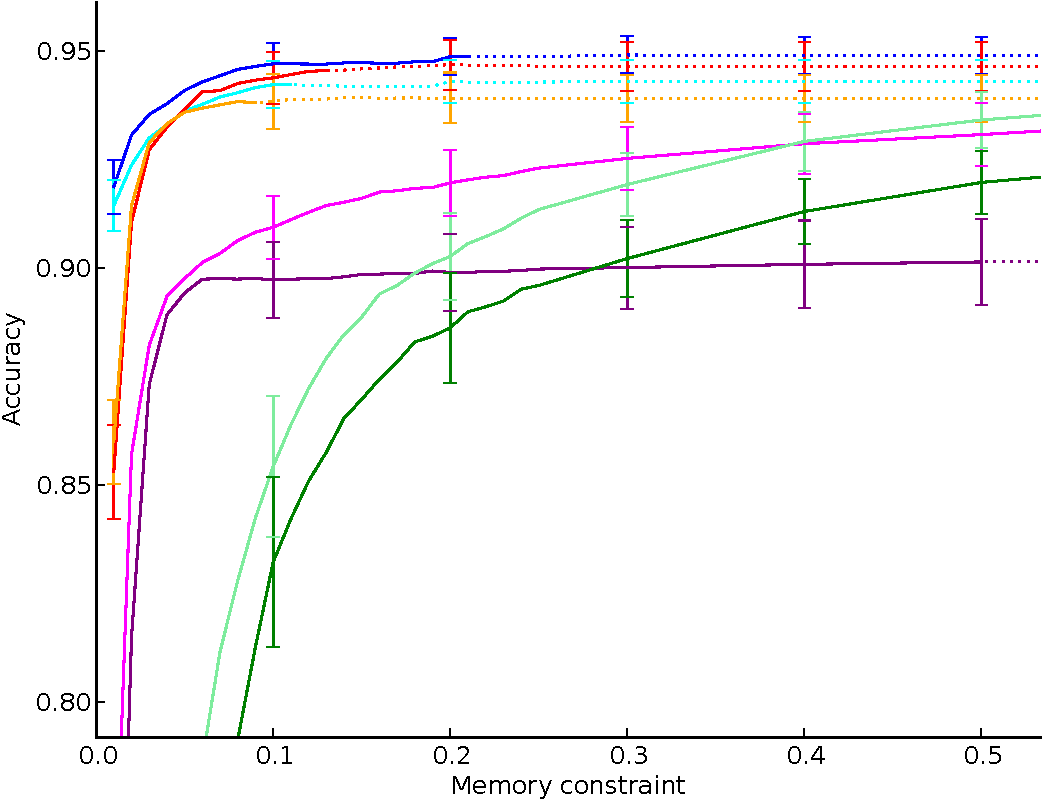
\includegraphics[width=0.5\textwidth]{figures/ch8/figure5-e-isolet.pdf}
        }
        \subfloat[\textsc{mnist3vs8}]{
        \label{fig:memc:mnist}
            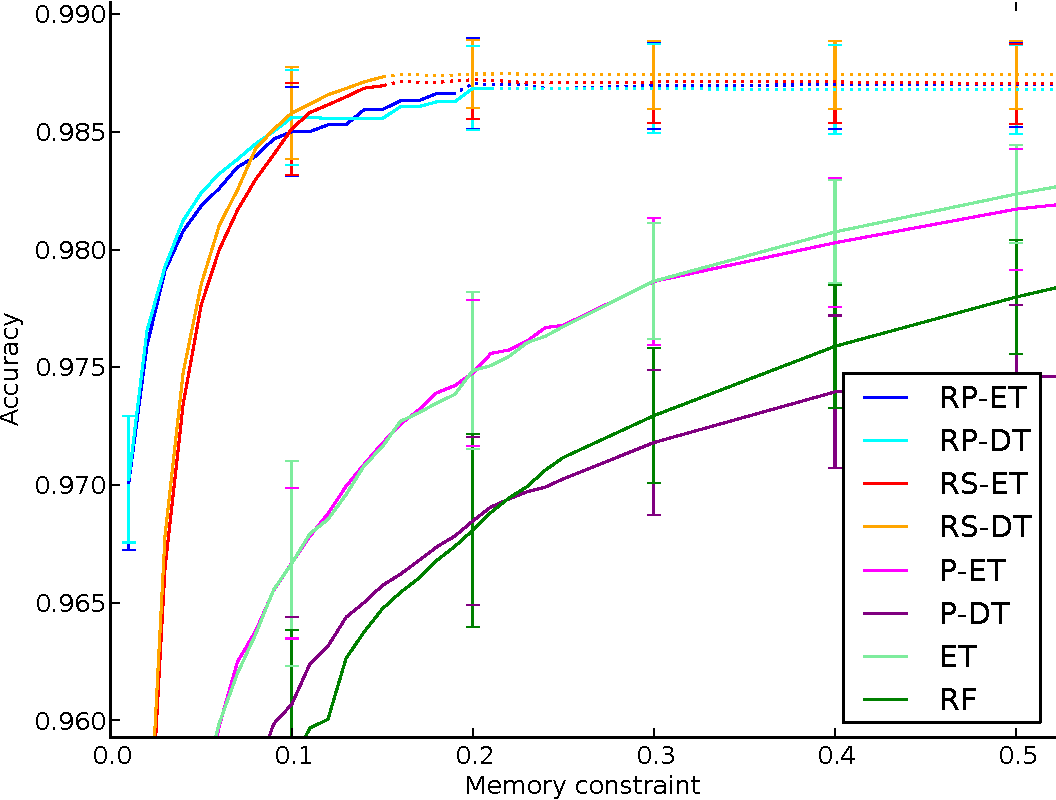
\includegraphics[width=0.5\textwidth]{figures/ch8/figure5-f-mnist.pdf}
        }
\caption{Accuracy under memory constraint.}
\label{fig:9:memc}
\end{center}
\end{figure}

To illustrate our point, Figure~\ref{fig:9:memc} compares for 6 representative
datasets the accuracy of the methods with respect to the memory constraint $\alpha_s
\alpha_f < \mu'_{\text{max}}$.  A plain line indicates that the generalization error of the
best resulting ensemble under memory constraint $\mu'_{\text{max}}$ is significantly (at $\alpha=0.05$)
worse on the test sets than when there is no constraint
(i.e., $\mu'_{\text{max}}=1$). A dotted line indicates that on average, on the test set, the
ensemble is not significantly less accurate.

As the figure shows, when $\mu'_{\text{max}}$ is low, RP-based ensembles often achieve
the best accuracy. Only on \textsc{arcene} (Figure~\ref{fig:memc:arcene}), RS seems to be a
better strategy, suggesting some overfitting in setting $\alpha_s$ in RP. On all 5
other example datasets, RP is equivalent or better than RS and P for low values
of $\mu'_{\text{max}}$, with the largest gaps appearing on \textsc{isolet}
(Figure~\ref{fig:memc:isolet}) and \textsc{mnist3vs8} (Figure~\ref{fig:memc:mnist}). As
already observed in the previous section, although RP-DT is not the best
strategy when memory is unconstrained, its curve dominates the curve of RP-ET
for small values of $\mu'_{\text{max}}$ in Figures \ref{fig:memc:cifar10},
\ref{fig:memc:tis}, and \ref{fig:memc:madelon}. Because split thresholds are
not randomized in RP-DT, this method is more resistant than RP-ET to the strong
randomization induced by a very low $\mu'_{\text{max}}$ threshold.

For comparison, Figure~\ref{fig:9:memc} also features the learning curves of both
ET and RF (with $K$ optimized on the validation set), in which the trees have
all been built on the {\it same} training sample of $\mu'_{\text{max}}N$ instances,
with all features. These results are representative of the use of a
straightforward sub-sampling of the instances to handle the memory constraint.
On all datasets, this setting yields very poor performance when $\mu'_{\text{max}}$ is
low. Building base estimators on re-sampled random patches thus brings a clear advantage to RP, RS and P and hence confirms the conclusions of \citet{basilico:2011} who showed that using more data indeed produces
more accurate models than learning from a single sub-sample.
This
latter experiment furthermore shows that the good performances of RP
cannot be trivially attributed to the fact that our datasets contain so many
instances that only processing a sub-sample of them would be enough. On most
problems, the slopes of the learning curves of RF and ET indeed suggest that
convergence has not yet been reached on these datasets. Yet, important
improvement are gained by sub-sampling random patches.
Contrary to intuition, it
also does not appear that the bigger the datasets, the lower $\mu'_{\text{max}}$ can be
reduced without loss of accuracy. Indeed, we found no conclusive correlation
between the size $Np$ of the dataset and the minimum value of $\mu'_{\text{max}}$ to
reach good performance\footnote{Spearman's rank correlation coefficient is
-0.0354 ($p-\mathrm{value}=0.8550$).}.
Overall, these results thus indicate that
building an ensemble on random patches is not only a good strategy when data is
abundant and redundant but also that it works even for scarce datasets with
limited information regarding the problem.

\subsection{Conclusions}

We have shown in this section that the memory requirements of sampling-based
ensembles are intrinsically low. Better, we have shown that they can often be
drastically decreased without significant loss in accuracy. When the size of the
dataset is far bigger than the available memory, we have also demonstrated that
sampling data along both samples and features, as RP does, not only competes
with other ensemble algorithms but also significantly improves the accuracy of
the resulting ensemble. It also brings a significant improvement over a
straightforward sub-sampling of the instances.

\section{Overall conclusions}
\label{sec:9:conclusions}

The main contribution of this work is to explore a new framework for supervised
learning in the context of very strong memory constraints or, equivalently, very
large datasets. To address such problems, we proposed the Random Patches
ensemble method that builds each individual model of the ensemble from a random
patch of the dataset obtained by drawing random subsets of both samples and
features from the whole dataset. Through extensive experiments with tree-based
estimators, we have shown that this strategy works as well as other popular
randomization schemes in terms of accuracy (Section~\ref{sec:9:accuracy}), at the
same time reduces very significantly the memory requirements to build each
individual model (Section~\ref{sec:9:memory:noloss}), and, given its flexibility,
attains significantly better accuracy than other methods when memory is severely
constrained (Section~\ref{sec:9:memory:loss}). Since all models are built
independently of each other, the approach is furthermore trivial to parallelize.
All in all, we believe that the paradigm of our method highlights a very promising
direction of research to address supervised learning on big data.

There remain several open questions and limitations to our approach that we
would like to address in the future. First, this study motivates our interest in
experimenting with truly large-scale problems (of giga-scale and higher). Since
RP already appears advantageous for small to medium datasets, the potential benefits on
very large-scale data indeed look very promising.

Second, the conclusions drawn in sections~\ref{sec:9:accuracy} and
\ref{sec:9:memory} are all based on the optimal values of the parameters $\alpha_s$ and
$\alpha_f$ tuned through an exhaustive grid search on the validation set. Our
analysis did not account for the memory and time required for tuning these two
parameters. In practice, hyper-parameter tuning can not be avoided as we have
shown that the optimal trade-off between $\alpha_f$ and $\alpha_s$ was problem dependent.
It would therefore be interesting to design an efficient strategy to
automatically find and adjust the values of $\alpha_s$ and $\alpha_f$, taking into account
the global memory constraint. Our simplistic framework also only accounts for
the memory required to store the training set in memory and not for the total
memory required to actually build the ensemble.

We have only explored uniform sampling of patches of fixed size in our
experiments. In the context of the Pasting approach, Breiman proposed
an iterative instance weighting scheme that proved to be more
efficient than uniform sampling \citep{breiman:1999}. It would be
interesting to extend this approach when sampling both instances and
features. Yet, parallelization would not be trivial anymore, although
probably still possible in the line of the work in \citep{chawla:2004}.

Finally, our analysis of RP is
mostly empirical. In the future, we would like to strengthen these
results with a more theoretical analysis. A starting point could be
the work in \citep{zinkevich:2010} that studies a scheme similar to the
Pasting method applied to linear models trained through parallel
stochastic gradient descent. The extension of this work to non
parametric tree-based estimators does not appear trivial however,
since these latter are not well characterized
theoretically.
